% NeurIPS 2026 Submission
\documentclass{article}

% NeurIPS style -- [preprint] for a clean one-column draft, [final] for camera-ready.
\usepackage[preprint,nonatbib]{neurips_2026}

\PassOptionsToPackage{table}{xcolor}
\usepackage[utf8]{inputenc}
\usepackage[T1]{fontenc}
\usepackage[breaklinks,colorlinks]{hyperref}
\usepackage{url}
\usepackage{booktabs}
\usepackage{amsmath}
\usepackage{amsfonts}
\usepackage{amssymb}
\usepackage{nicefrac}
\usepackage{microtype}
\usepackage{graphicx}
\usepackage{multirow}
\usepackage{tabularx}
\usepackage{xcolor}
\usepackage{colortbl}
\usepackage{subcaption}
\usepackage{float}
\usepackage{placeins}
\floatstyle{ruled}
\newfloat{algobox}{tbp}{loa}
\floatname{algobox}{Algorithm}

\newcounter{algorithm}
\newenvironment{cvpralgorithm}{\begin{figure}[!htbp]\refstepcounter{algorithm}\noindent\begin{minipage}{\linewidth}}{\end{minipage}\end{figure}}
\newcommand{\algorithmcaption}[1]{\noindent\emph{Algorithm \thealgorithm. #1}\par\vspace{2pt}}
\newcommand{\algkw}[1]{\emph{#1}}
\newcommand{\algindent}{\hspace*{1.2em}}
\newcommand{\algindenttwo}{\hspace*{2.4em}}
\newcommand{\etal}{\emph{et al.}}

\title{Depth Conditioned Feature Composting for Unsupervised Monocular Panoptic Segmentation}

\author{Anonymous Author(s)}

\begin{document}
\raggedbottom

\maketitle

\begin{abstract}
Existing unsupervised panoptic methods for full driving scenes rely on calibrated stereo and unsupervised optical flow, which excludes the long tail of monocular footage from phones, dashcams, and fixed cameras. The redundancy that stereo and motion previously supplied is recoverable from agreement among single-frame priors. On this principle we introduce two compact mechanisms: DCFA, a residual adapter ($\sim$225K parameters) that conditions a frozen unsupervised semantic code on monocular depth, and SIMCF, a learning-free filter that enforces semantic, geometric, and appearance agreement on candidate panoptic labels. Trained on raw monocular pseudo-labels, the adopted CUPS~\cite{hahn2025cups} panoptic trainer reaches 32.76 PQ on Cityscapes val; DCFA and SIMCF lift the same trainer to 35.83 PQ, a contribution-isolated $+$3.07 PQ over the matched monocular baseline. The +5.0 PQ gap between this baseline (32.76) and the published CUPS stereo+flow configuration (27.80) reflects the pseudo-label-source substitution alone.
\end{abstract}

%=========================================================================
\section{Introduction}
\label{sec:intro}
%=========================================================================

Most driving footage that ingests into perception pipelines, including phone video, dashcam captures, and fixed-camera streams, is monocular. Supervised panoptic segmentation dominates benchmarks but requires dense per-instance annotation that does not scale across datasets and domains. The unsupervised setting asks whether panoptic structure can be recovered from raw pixels alone, and current scene-centric methods answer this only when stereo and motion cues are available at pseudo-label time.

Three lineages partially answer this question: self-supervised semantic discovery on frozen DINO features~\cite{oquab2024dinov2,kim2024cause}, cut-and-learn instance discovery~\cite{wang2023cutler}, and 3-D depth-graph cuts for instance separation~\cite{sick2025cuts3d}. Their scene-centric synthesis is CUPS~\cite{hahn2025cups}, which combines semantic pseudo-labels with stereo-derived depth and unsupervised scene flow, then trains a Cascade Mask R-CNN with DropLoss bootstrapping and EMA self-training. CUPS achieves the current state of the art on Cityscapes only when stereo and motion cues are available at pseudo-label time; for monocular footage, the construction simply does not run.

We show that frozen monocular priors are sufficient when composed through cross-modal agreement, recovering the redundancy that stereo and motion previously supplied. Each prior fails on its own: semantic codes merge adjacent same-class objects or split surfaces under illumination change; monocular depth exposes physical separations but over-fragments along material seams; dense feature similarity merges depth fragments whose appearance is compatible. Our pipeline uses these failure modes against each other: depth proposes candidate boundaries, while semantic identity and feature similarity decide which boundaries survive. We make three contributions:
\begin{itemize}
\item \textbf{Monocular pseudo-label pipeline} that removes calibrated stereo and unsupervised optical flow from the CUPS~\cite{hahn2025cups} pseudo-label construction, replacing them with frozen single-frame priors composed through cross-modal agreement.
\item \textbf{Two compact mechanisms} for that composition: DCFA, a $\sim$225K-parameter residual adapter that conditions a frozen unsupervised semantic code on monocular depth; and SIMCF, a learning-free filter that enforces semantic, geometric, and appearance agreement on candidate panoptic labels.
\item \textbf{Contribution-isolated improvement on Cityscapes} under the CUPS~\cite{hahn2025cups} evaluation protocol: $+$3.07 PQ over a matched monocular baseline that shares our Stage-2 trainer and DINOv3 ViT-B/16 backbone (Table~\ref{tab:main}). Final 35.83 PQ surpasses the published stereo+flow CUPS configuration; we attribute the headline gap to both monocular pseudo-label substitution and our two mechanisms, with the controlled comparison isolating the latter.
\end{itemize}

\begin{figure}[!htbp]
\centering
\includegraphics[width=\textwidth]{../figures/paper_ready/pipeline_overview.png}
\caption{Pipeline overview. Stage 1 constructs panoptic pseudo-labels from a \emph{single RGB image} using frozen semantic features, monocular depth, DCFA, and SIMCF; the entire pipeline runs without stereo, optical flow, or any temporal neighbours. Stage 2 adopts CUPS-style~\cite{hahn2025cups} panoptic bootstrapping and panoptic network training on the filtered labels.}
\label{fig:pipeline_overview}
\end{figure}

%=========================================================================
\FloatBarrier
\section{Related Work}
\label{sec:related}
%=========================================================================

We position our work against three lines of unsupervised segmentation literature, each addressing one of the three lineages identified in Section~\ref{sec:intro}: semantic clustering with depth, cut-and-learn instance discovery, and scene-centric panoptic synthesis.

\paragraph{Unsupervised Semantic Segmentation with Depth.}
Unsupervised semantic segmentation has migrated from clustering-based objectives~\cite{ji2019iic,cho2021picie} to distillation on top of self-supervised ViT features~\cite{caron2021dino,oquab2024dinov2}, with STEGO~\cite{hamilton2022stego}, HP~\cite{seong2023hp}, and CAUSE~\cite{kim2024cause} producing dense semantic codes; recent refinements~\cite{kim2024eagle,seong2024ppap,couairon2024diffcut,bonnet2024hierarchy} sharpen the clustering objective without changing the substrate. Monocular depth has been used as an auxiliary signal in DepthG~\cite{sick2024depthg}, in CUPS~\cite{hahn2025cups}, and as multi-task pretraining~\cite{hoyer2021threeways}; supervised RGB-D fusion~\cite{yin2025dformerv2} requires dense labels. DCFA differs along two axes: \emph{conditioning site} (a feature-level residual adapter on a frozen clusterbook code, $\sim$225K trainable parameters, vs.\ end-to-end backbone updates in DepthG) and \emph{what is conditioned} (an already-trained, frozen unsupervised code, preserved on its original manifold). This positions DCFA distinctly within the broader adapter literature. Weight-level approaches such as LoRA~\cite{hu2022lora}, Houlsby~\cite{houlsby2019adapter} and AdaptFormer~\cite{chen2022adaptformer} decompose frozen layer weights, while cross-modal feature adapters such as FiLM~\cite{perez2018film}, CLIP-Adapter~\cite{gao2023clipadapter} and VL-Adapter~\cite{sung2022vladapter} use affine modulation or single-modality residuals. DCFA instead injects a cross-modal residual MLP into a frozen unsupervised semantic code, with zero-init identity bootstrapping and a $\lambda_p{=}20$ preserve loss. The FiLM versus concat$+$MLP design choice is ablated in Table~\ref{tab:conditioning}.

\paragraph{Unsupervised Instance Segmentation.}
The dominant line applies graph-cut-style partitioning to self-supervised features: LOST~\cite{simeoni2021lost}, TokenCut~\cite{wang2023tokencut}, MaskCut and CutLER~\cite{wang2023cutler}, MaskDistill~\cite{vangansbeke2022maskdistill}, and FreeSOLO~\cite{wang2022freesolo} establish the cut-and-learn template. Recent extensions diversify it with multi-SSL voting (CuVLER~\cite{arica2024cuvler}), single-pass cutting (COLER~\cite{feng2025coler}), prompt-and-merge (ProMerge~\cite{li2024promerge}), boundary-field learning (unMORE~\cite{yang2025unmore}), granularity-controlled SA-1B-scale segmentation (UnSAM/UnSAMv2~\cite{wang2024unsam,yu2025unsamv2}), and slot-attention object discovery (DINOSAUR~\cite{seitzer2023dinosaur}, MR-DINOSAUR~\cite{gong2025mrdinosaur}). The closest comparison to our instance pipeline is CutS3D~\cite{sick2025cuts3d}, which lifts depth to a 3-D point cloud and applies LocalCut on a 3-D k-NN graph. We share CutS3D's monocular premise but stay entirely in 2-D: depth gradients provide a 2-D proxy for the same physical-separation cue, supplied via Sobel filtering and connected-component analysis within thing-eligible semantic regions, without lifting to a 3-D graph.

\paragraph{Unsupervised Panoptic Segmentation.}
Three works frame the current scene-centric Cityscapes~\cite{cordts2016cityscapes} literature. U2Seg~\cite{niu2024u2seg} introduced the first unified unsupervised framework for combined semantic and instance segmentation, composing STEGO-style semantic features with MaskCut instance proposals on object-centric pretraining data and transferring the resulting model to scene-centric benchmarks. CUPS~\cite{hahn2025cups} established the current scene-centric state of the art by constructing pseudo-labels from stereo video, unsupervised optical flow~\cite{stone2021smurf}, and SF2SE3 scene-flow segmentation~\cite{sommer2022sf2se3}, then training a Cascade Mask R-CNN with DropLoss bootstrapping followed by three rounds of EMA self-training. S2-UniSeg~\cite{xu2025s2uniseg} proposed a single-stage monocular alternative based on segmentation-oriented pretraining at the SA-1B scale ($\sim$11M images) followed by adaptation to the target dataset, removing the multi-stage pseudo-label pipeline at the cost of a larger pretraining corpus.



%=========================================================================
\section{Method}
\label{sec:method}
%=========================================================================

\subsection{Problem Setup and Pipeline Overview}
\label{sec:method:setup}

We address scene-centric unsupervised panoptic segmentation in the monocular variant of the CUPS setting~\cite{hahn2025cups}: training is given an unlabeled image set $\mathcal{D}_{\text{train}} = \{x_i\}_{i=1}^{N}$ where each $x_i \in \mathbb{R}^{H \times W \times 3}$ is a single RGB frame from the target dataset, here Cityscapes~\cite{cordts2016cityscapes}. No annotations, ground-truth or sensor depth, calibrated stereo, or temporal neighbours are available; only frozen off-the-shelf visual and depth priors are used. The two stages are
\begin{equation}
G(x) = (\hat S_x, \hat I_x), \qquad F(x) = (S_x, I_x),
\label{eq:pipeline}
\end{equation}
where $G$ is the monocular pseudo-label generator used during training and $F$ is the panoptic network evaluated at test time. The maps $\hat S_x$ and $S_x$ assign semantic labels to pixels, while $\hat I_x$ and $I_x$ assign instance identities to pixels belonging to countable object classes.

Figure~\ref{fig:pipeline_overview} summarizes the two-stage pipeline: Stage 1 fits a generator on unlabeled target images and applies it per-frame; Stage 2 follows the CUPS~\cite{hahn2025cups} panoptic bootstrapping and EMA self-training procedures on the resulting pseudo-labels. Holding Stage 2 fixed attributes any change in final performance to the pseudo-label source.

The Stage-1 generator builds on two frozen, target-annotation-free priors, a DINOv2 ViT-B/14 backbone~\cite{oquab2024dinov2} and the CAUSE-TR head~\cite{kim2024cause}, augmented by two trainable or learning-free modules introduced in this paper: the Depth-Conditioned Feature Adapter (DCFA, Section~\ref{sec:method:dcfa}) and the SIMCF filter (Section~\ref{sec:method:simcf}). The semantic branch produces $\hat S_x$ by passing $x$ through the frozen backbone and CAUSE-TR head to obtain a 90-dimensional code, refined by DCFA before clustering. The instance branch produces $\hat I_x$ from Sobel responses on a monocular depth map, restricted to thing-eligible semantic regions. SIMCF then filters the candidate labels by checking semantic identity, instance geometry, and feature similarity.


\subsection{Monocular Pseudo-Label Baseline}
\label{sec:method:baseline}

\begin{figure}[!htbp]
\centering
\begin{subfigure}{\textwidth}
\centering
\includegraphics[width=\textwidth]{../figures/paper_ready/pseudo_label_generation.png}
\caption{Pseudo-label generation. The semantic branch clusters depth-conditioned CAUSE-TR~\cite{kim2024cause} codes; the instance branch converts monocular depth gradients into connected components inside thing-eligible regions; SIMCF filters candidate labels.}
\label{fig:pseudolabel_generation}
\end{subfigure}\\[2pt]
\begin{subfigure}{0.7\linewidth}
\centering
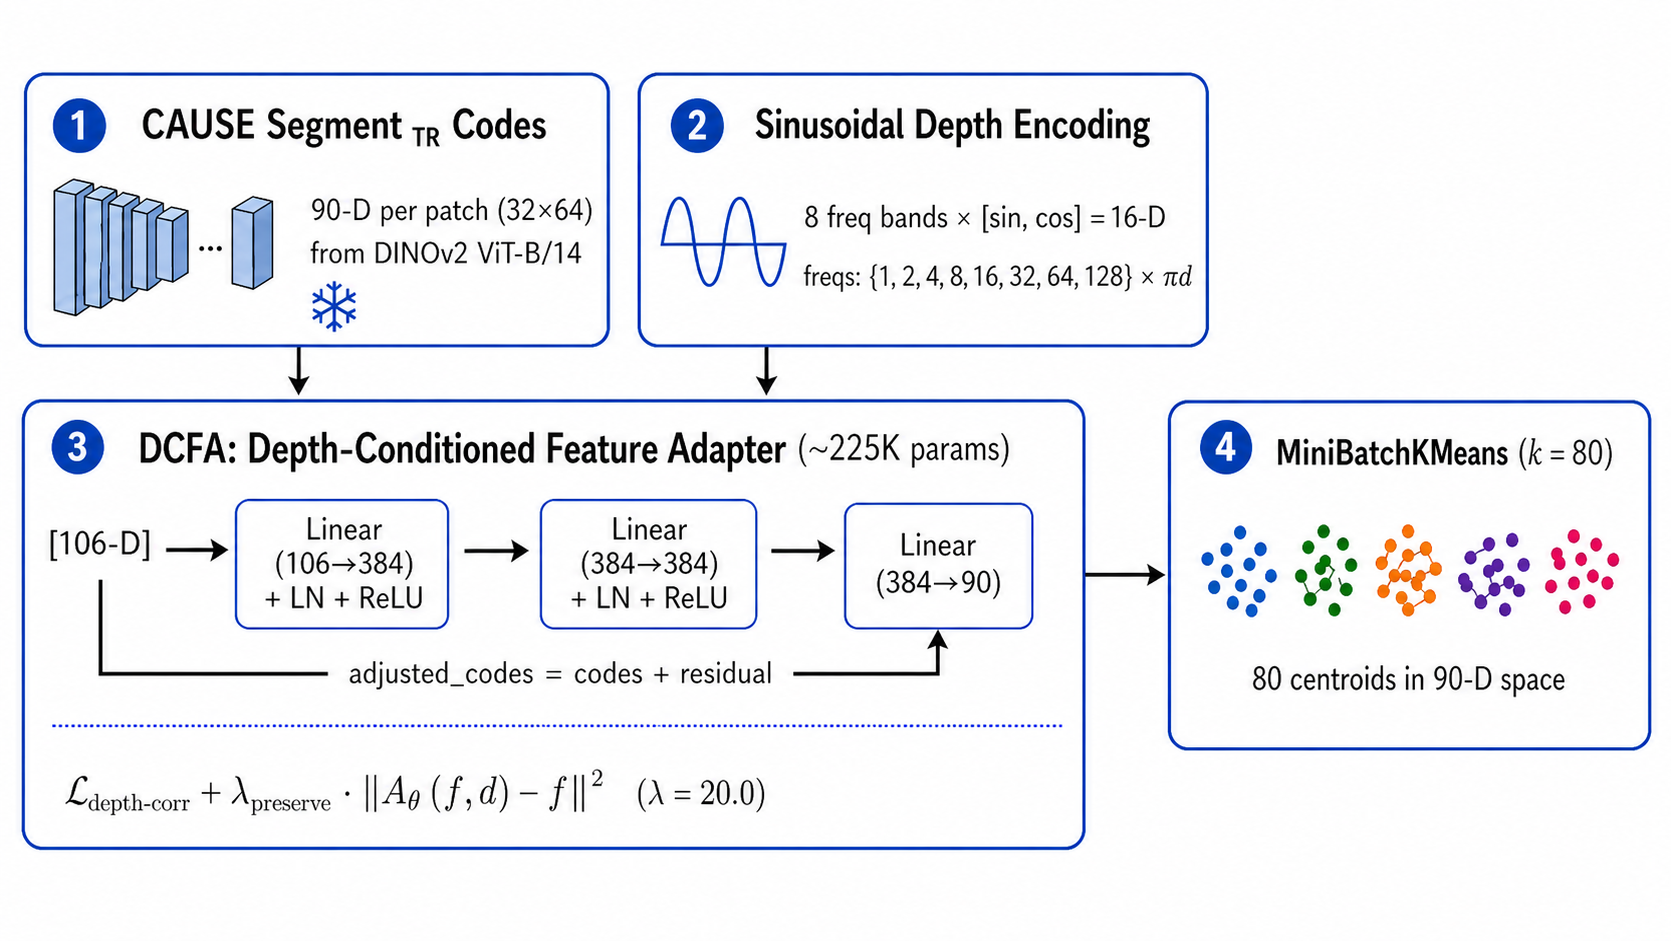
\includegraphics[width=\linewidth]{../figures/paper_ready/dcfa_adapter_training.png}
\caption{DCFA adapter training. A frozen CAUSE-TR code is adjusted by a depth-conditioned residual before $k$-means clustering, with a preservation term keeping the adapted code on the original frozen semantic manifold.}
\label{fig:dcfa_adapter}
\end{subfigure}
\caption{Stage-1 pipeline. (a) End-to-end pseudo-label generation. (b) DCFA adapter training detail.}
\label{fig:stage1}
\end{figure}

Monocular depth exposes the same physical-separation cues that stereo and scene flow give CUPS~\cite{hahn2025cups}, provided the discontinuity is read at the right spatial scale and only within a region whose semantic identity has been estimated. Figure~\ref{fig:stage1}(a) shows how the semantic and depth branches provide the raw candidate labels that SIMCF later filters.

The semantic branch is assembled entirely from frozen priors. Each image $x$ is encoded by a frozen DINOv2 ViT-B/14 backbone~\cite{oquab2024dinov2}, whose dense patch features are then reduced by a frozen CAUSE-TR head~\cite{kim2024cause} to a 90-dimensional semantic code. We L2-normalize these codes and partition them with k-means on the unlabeled training set into $k = 80$ centroids, assigning each pixel the index of its nearest centroid to obtain $\hat S_x$. The cardinality $k = 80$ is deliberately well above the 27-class evaluation taxonomy: collapsing to 27 classes at this stage would erase fine visual modes that the depth-based instance branch later relies on. CUPS reports that this regime monotonically improves panoptic quality as $k$ exceeds the evaluation cardinality~\cite{hahn2025cups}.

With $\hat S_x$ in hand, the instance branch reads physical-separation structure from a single monocular depth map $D \in \mathbb{R}^{H \times W}$. We use a frozen DepthPro network~\cite{bochkovskii2024depthpro}, chosen because it balances boundary sharpness against surface smoothness; an empirical comparison against SPIdepth and DA3 is reported in Table~\ref{tab:depth}. We first apply a small Gaussian smoothing kernel to $D$ to suppress sub-pixel depth noise, then convolve with $3 \times 3$ Sobel kernels $K_u, K_v$ along the spatial axes and flag candidate boundaries by thresholding the resulting gradient magnitude,
\begin{equation}
\begin{aligned}
g_D(p) &= \sqrt{(K_u * D)^2(p) + (K_v * D)^2(p)}, \\
B_D(p) &= \mathbf{1}\{g_D(p) > \tau_d\}, \qquad \tau_d = 0.20 .
\end{aligned}
\label{eq:depth_boundary}
\end{equation}
Pixels with $B_D(p)=1$ are flagged as candidate boundaries. We set $\tau_d = 0.20$ using label-free pseudo-instance statistics; sharper thresholds over-fragment the training data, as discussed alongside Table~\ref{tab:depth}. Connected-component labelling with 8-neighbour adjacency is run only inside thing-eligible semantic regions. Each of the 80 over-clusters is assigned to its nearest concept in the CAUSE~\cite{kim2024cause} 27-class self-supervised vocabulary by centroid distance in the 90-dimensional code space, and thing-eligibility is read off the CAUSE taxonomy~\cite{kim2024cause} (eight countable categories). This over-cluster-to-concept map $\phi$ is computed entirely from frozen self-supervised features and uses no ground-truth labels; a precise specification is given in Appendix~\ref{sec:supp:impl:phi}. Components below $A_\text{min} = 1000$ pixels are discarded, and the surviving components are dilated with three iterations of a $3 \times 3$ structuring element. We denote the resulting raw candidate pseudo-labels $(S_x^0, I_x^0)$, where $S_x^0 = \hat S_x$ holds the over-cluster semantic map and $I_x^0$ holds the connected-component instance map; SIMCF (Section~\ref{sec:method:simcf}) consumes this pair.

The semantic regions inherited from the frozen CAUSE-TR~\cite{kim2024cause} code are appearance-driven and can split a single physical surface across an illumination change or merge two adjacent same-class objects. Closing this gap requires conditioning the semantic code on the same depth signal that already governs the instance branch.


\subsection{Depth-Conditioned Feature Adapter (DCFA)}
\label{sec:method:dcfa}

Figure~\ref{fig:stage1}(b) summarizes the adapter path. We introduce a small residual adapter that consumes the depth value $d_u$ at pixel $u$ and adds a learned depth-driven shift to the frozen 90-dimensional code $z_u$, nudging cluster boundaries toward depth-consistent regions where appearance fails.

Conditioning on $d_u$ requires a representation rich enough for a small MLP to read both fine boundary differences and coarse depth ordering. Since $d_u \in [0, 1]$ is a scalar, we lift it through a 16-dimensional sinusoidal positional encoding with eight exponentially-spaced frequencies $\omega_k = 2^k \pi$ for $k = 0, \dots, 7$,
\begin{equation}
\begin{aligned}
e(d_u) = \big[ &\sin(\omega_0 d_u), \cos(\omega_0 d_u), \dots, \\
              &\sin(\omega_7 d_u), \cos(\omega_7 d_u) \big] \in \mathbb{R}^{16}.
\end{aligned}
\label{eq:sinusoid}
\end{equation}
The encoding $e(d_u)$ is concatenated with the frozen 90-dimensional code $z_u$ and passed through a two-hidden-layer MLP $r: \mathbb{R}^{106} \to \mathbb{R}^{384} \to \mathbb{R}^{384} \to \mathbb{R}^{90}$ (hidden width $h = 384$, LayerNorm and ReLU after each hidden layer, zero-initialized output projection). The MLP produces a depth-conditioned shift that is added residually to the frozen code,
\begin{equation}
\tilde z_u = z_u + r\big([z_u; e(d_u)]\big).
\label{eq:residual}
\end{equation}
The construction has approximately 225K trainable parameters (0.26\% of the $\sim$86M-parameter frozen ViT backbone). Zero initialisation of the output projection makes $\tilde z_u = z_u$ at step 0, so any departure from the frozen code is acquired gradually under the loss below.

Training applies the DepthG~\cite{sick2024depthg} depth-feature correlation loss to the adapted code rather than to the backbone weights, paired with a preservation term that penalises drift from $z_u$ and keeps $\tilde z$ on the original CAUSE-TR~\cite{kim2024cause} manifold. The adapter minimizes
\begin{equation}
\begin{aligned}
\mathcal{L}_\text{DCFA}
&= \mathcal{L}_\text{corr}(\tilde z, D)
 + \lambda_p \mathcal{L}_\text{preserve}(\tilde z, z), \\
\lambda_p &= 20 .
\end{aligned}
\label{eq:dcfa_loss}
\end{equation}
The preservation weight $\lambda_p = 20$ was selected from a sweep over $\{1, 5, 10, 20, 50\}$ on the unlabeled training set such that the preservation term dominates outside high-similarity neighbourhoods (Appendix~\ref{sec:supp:impl}).
$\mathcal{L}_\text{corr}$ is the DepthG~\cite{sick2024depthg} depth-similarity-weighted feature-correlation loss; $\mathcal{L}_\text{preserve}$ is a per-pixel squared distance between $\tilde z_u$ and the frozen $z_u$. Formal definitions and sampling details are in Appendix~\ref{sec:supp:impl}.
\subsection{SIMCF: Semantic Instance Mutual Consistency Filtering}
\label{sec:method:simcf}

DCFA changes the feature space before clustering, but residual errors persist: a depth fragment may cut through a single object, a proposal may mix pseudo-classes, or a semantic assignment may sit at a depth far from its pseudo-class range. SIMCF (Semantic Instance Mutual Consistency Filtering) is the final algorithm inside $G$: it maps the raw candidate pair $(S_x^0, I_x^0)$ to filtered pseudo-labels $(\hat S_x, \hat I_x)$ by enforcing consistency across semantic identity, instance geometry, feature similarity, and depth statistics.

SIMCF runs three sequential checks. \textbf{(A)} For each instance region, the dominant pseudo-class is identified and within-region pixels of conflicting classes are reassigned, preventing mixed-class instance targets. \textbf{(B)} Adjacent proposal pairs whose mean DINOv3 features~\cite{simeoni2025dinov3} agree above $\tau_\text{sim}$ and whose dominant classes match are merged, repairing depth over-fragmentation. We use DINOv3 features here because the appearance-similarity check benefits from the slightly stronger off-the-shelf descriptor, while the rest of Stage-1 stays on the DINOv2-trained CAUSE-TR clusterbook to preserve compatibility with the frozen 90-D code. \textbf{(C)} Pixels whose depth lies more than $\eta\sigma_c$ from the per-class depth mean are reassigned to void rather than treated as hard negatives. SIMCF is learning-free; the two SIMCF-specific hyperparameters are $\tau_\text{sim}$ and $\eta$. The depth-branch parameters $A_\text{min}$ (minimum component area) and 8-neighbour adjacency, introduced in Section~\ref{sec:method:baseline}, are also fixed across all experiments. The over-cluster-to-concept map $\phi$ is the same construction defined in Section~\ref{sec:method:baseline}; a precise no-ground-truth specification is given in Appendix~\ref{sec:supp:impl:phi}.

\begin{figure}[!htbp]
\centering
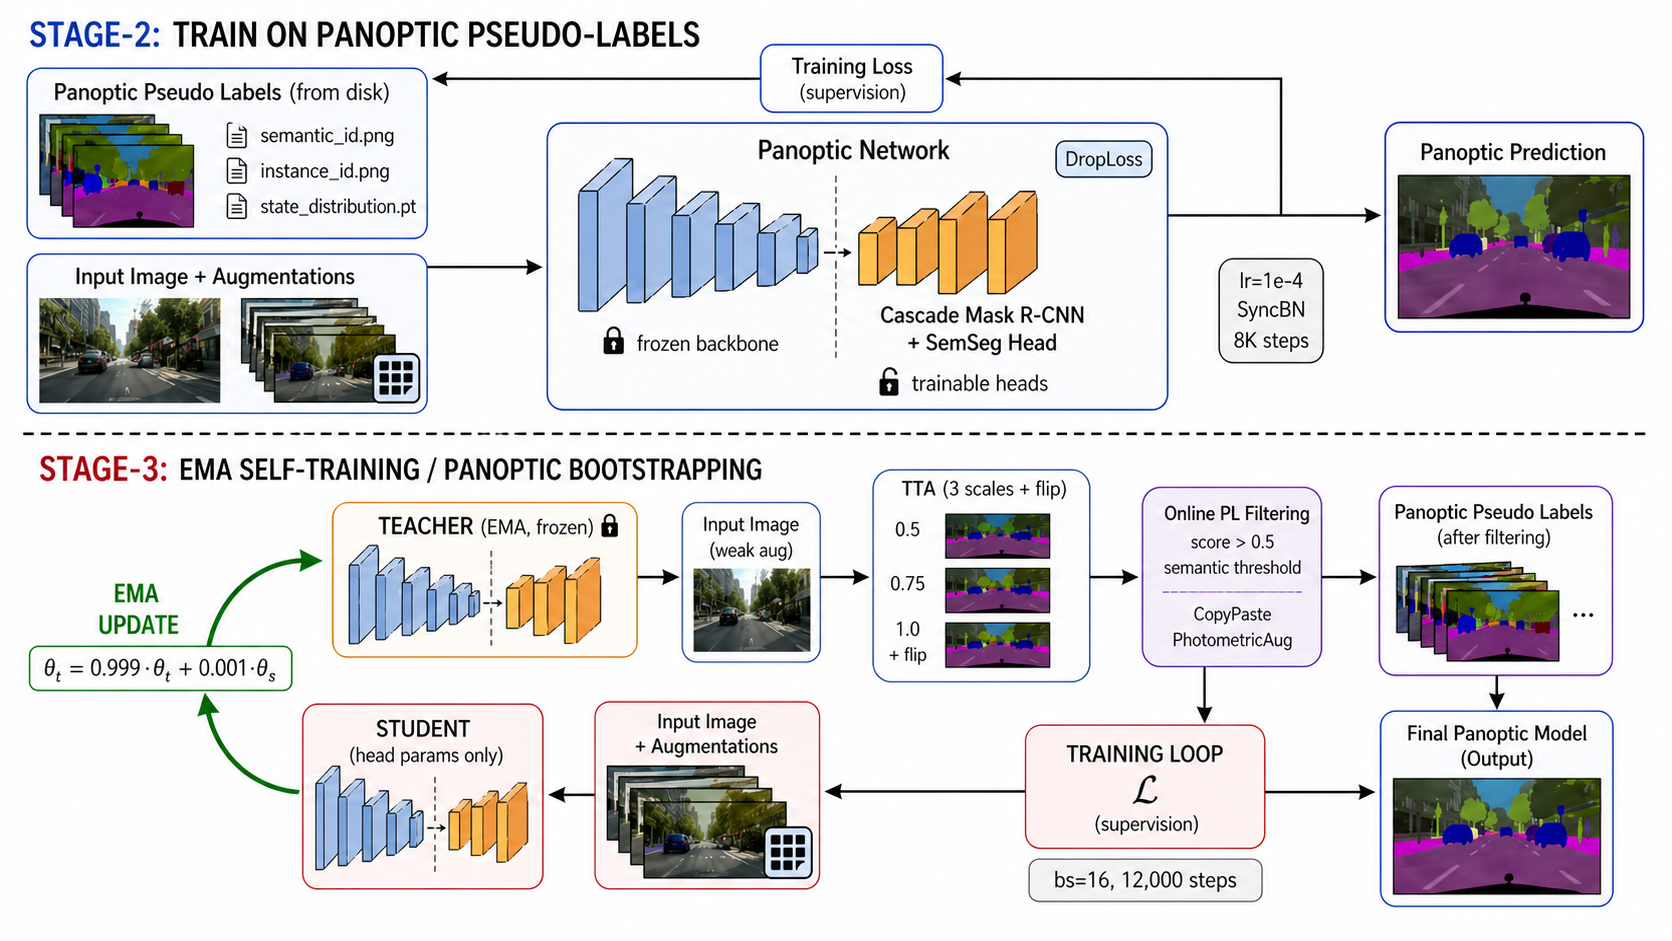
\includegraphics[width=0.90\textwidth]{../figures/paper_ready/panoptic_network_training.png}
\caption{Panoptic bootstrapping and panoptic network training. Filtered pseudo-labels supervise the initial panoptic network, and EMA self-training refines the labels and network across subsequent rounds, following the CUPS~\cite{hahn2025cups} training recipe.}
\label{fig:panoptic_training}
\end{figure}

\subsection{Panoptic Bootstrapping and Panoptic Network Training}
\label{sec:method:detector}

Filtering completes the Stage-1 generator $G$. We adopt the panoptic bootstrapping and EMA self-training procedures of CUPS~\cite{hahn2025cups} verbatim and use the final-round student as the network $F$ in Eq.~\ref{eq:pipeline}. Four CUPS components carry distinct roles in this stage: Cascade Mask R-CNN heads provide multi-stage IoU refinement against the noisy pseudo-label boundaries; DropLoss~\cite{wang2023cutler} masks the loss on void regions so that rejected SIMCF pixels are not treated as hard negatives; self-enhanced copy-paste augmentation mitigates the long-tail class imbalance present in the 80-cluster pseudo-vocabulary; and three rounds of EMA self-training iteratively denoise the pseudo-labels using the network's own predictions as a teacher. The detector backbone is a frozen DINOv3 ViT-B/16~\cite{simeoni2025dinov3}, kept frozen across all configurations to keep capacity fixed and prevent backbone confounds with the pseudo-label-source ablation. Holding these procedures fixed lets the experiments isolate the effect of the pseudo-label source. Figure~\ref{fig:panoptic_training} shows the training path; full hyperparameters are in Section~\ref{sec:exp:setup} and Appendix~\ref{sec:supp:impl}.

At test time, $F$ produces $(S_x, I_x)$ via the standard panoptic merge~\cite{kirillov2019panoptic}. Two non-obvious design choices: (i) $F$ predicts directly into the pseudo-class vocabulary it was trained on; the Hungarian map to the 27-class Cityscapes~\cite{cordts2016cityscapes} taxonomy is computed only at evaluation time and is the only ground-truth-derived component anywhere in the pipeline. (ii) The thing/stuff partition driving the merge is inherited from the frozen CAUSE-TR~\cite{kim2024cause} taxonomy, so the same partition supervises Stage-1 instance extraction and test-time panoptic merging without taxonomy drift.

%=========================================================================
\FloatBarrier
\section{Experiments}
\label{sec:experiments}
%=========================================================================

We evaluate on Cityscapes~\cite{cordts2016cityscapes} and zero-shot transfer datasets, separating pseudo-label quality from trained-network performance and asking how much DCFA and SIMCF contribute and where the Cityscapes-derived pseudo-class vocabulary fails.

\subsection{Experimental Setup}
\label{sec:exp:setup}

Pseudo-label generation and panoptic network training use only Cityscapes train~\cite{cordts2016cityscapes} (2{,}975 images, no annotations); evaluation reports Cityscapes val (500 images) under the 27-class CAUSE~\cite{kim2024cause} pseudo-vocabulary with a Hungarian map to the 27-class Cityscapes label space (\texttt{NUM\_CLASSES=27} in the official CUPS protocol~\cite{hahn2025cups}, the full Cityscapes label space). The Stage-1 generator $G$ couples a frozen DINOv2 ViT-B/14 backbone~\cite{oquab2024dinov2} and CAUSE-TR head~\cite{kim2024cause} with DCFA ($h{=}384$, $\lambda_p{=}20$, $\sim$225K trainable parameters), $k$-means over-clustering at $k{=}80$, the monocular instance branch ($\tau_d{=}0.20$, $A_\text{min}{=}1000$), and SIMCF ($\tau_\text{sim}{=}0.85$, $\eta{=}2.5$); DepthPro~\cite{bochkovskii2024depthpro} supplies the monocular depth map. The panoptic network is a three-stage Cascade Mask R-CNN~\cite{cai2018cascade} on a frozen DINOv3 ViT-B/16 backbone~\cite{simeoni2025dinov3}, trained with CUPS-style~\cite{hahn2025cups} panoptic bootstrapping (8K steps, DropLoss~\cite{wang2023cutler}, copy-paste) followed by three 5K-step EMA self-training rounds. All operating hyperparameters were fixed before consulting Cityscapes annotations; the SIMCF sweep in Appendix~\ref{sec:supp:simcf_sweep} is a retrospective sensitivity analysis, not a model-selection procedure. Full hyperparameter recipes, optimizer schedules, augmentation lists, hardware, and wall-clock budgets are reported in Appendix~\ref{sec:supp:impl} of the supplementary material.


\subsection{Main Cityscapes Results}
\label{sec:exp:main}

Table~\ref{tab:main} records two comparisons on Cityscapes val: published external references and an in-paper controlled comparison holding the Stage-2/3 trainer fixed. The two ``ours'' rows isolate DCFA$+$SIMCF: both share the same Stage-2/3 recipe and DINOv3 ViT-B/16 backbone, differing only in the Stage-1 pseudo-label source. The monocular baseline is trained on raw $K{=}80$ pseudo-labels without DCFA or SIMCF (raw 90-D CAUSE-TR~\cite{kim2024cause} code; DepthPro connected components at $\tau_d{=}0.20$). Our method surpasses the published stereo+flow CUPS reference; the supervised row (62.3 PQ) is an oracle upper bound.

\begin{table}[!htbp]
\caption{Unsupervised panoptic segmentation on Cityscapes~\cite{cordts2016cityscapes} \textbf{val} (all in \%, $\uparrow$). ``PL inputs'' are the inputs available at pseudo-label time. ``Eval cls.'' is the number of benchmark classes used by the CUPS~\cite{hahn2025cups} evaluation protocol; our network predicts $K{=}80$ pseudo-classes and is aligned to the 27-class taxonomy only at metric time (Section~\ref{sec:exp:setup}). Tables in this main section report Cityscapes \textbf{val} numbers; ablation tables in Appendix C/D that report Cityscapes \textbf{train} pseudo-label PQ are flagged in their captions.}
\label{tab:main}
\centering
\small
\setlength{\tabcolsep}{3pt}
\resizebox{\textwidth}{!}{%
\begin{tabular}{l l l c c c c c c}
\toprule
Method & Training data & PL inputs & Eval cls. & PQ & SQ & RQ & PQ$^\text{Th}$ & PQ$^\text{St}$ \\
\midrule
\rowcolor{black!5} Supervised~\cite{kirillov2019panoptic} & CS & dense labels & -- & 62.3 & 81.8 & 75.1 & 62.4 & 62.1 \\
\midrule
DepthG~\cite{sick2024depthg}$+$CutLER~\cite{wang2023cutler} & CS \& ImageNet & RGB mono. & 27 & 16.1 & 45.4 & 21.1 & \phantom{0}3.0 & 25.7 \\
U2Seg~\cite{niu2024u2seg} & COCO \& ImageNet & RGB mono. & 800$+$27 & 18.4 & 55.8 & 22.7 & 10.2 & 24.3 \\
S2-UniSeg~\cite{xu2025s2uniseg} & SA-1B \& CS & RGB mono. & -- & 25.4 & 66.7 & 35.0 & -- & -- \\
CUPS~\cite{hahn2025cups} & CS & RGB$+$stereo$+$flow & 27 & 27.80 & 57.4 & 35.2 & 17.7 & 35.1 \\
\midrule
Monocular baseline (no DCFA/SIMCF) & CS & RGB mono. & 27 & 32.76 & 62.57 & 40.75 & -- & -- \\
\textbf{Ours (DCFA$+$SIMCF)} & CS & RGB mono. & 27 & \textbf{35.83} & \textbf{62.79} & \textbf{43.78} & \textbf{36.26} & \textbf{35.56} \\
\midrule
\textit{vs.\ CUPS~\cite{hahn2025cups}} (prev.\ scene-centric SOTA) & & & & \textcolor{green!50!black}{$+$8.03} & \textcolor{green!50!black}{$+$5.39} & \textcolor{green!50!black}{$+$8.58} & \textcolor{green!50!black}{$+$18.56} & \textcolor{green!50!black}{$+$0.46} \\
\bottomrule
\end{tabular}
}
\end{table}

The improvement over the pseudo-label generator is concentrated in recognition rather than mask quality, indicating that panoptic bootstrapping and EMA self-training principally amplify class recall while preserving the mask geometry already produced by the Stage-1 generator. The trained-model mIoU of 44.56\% (under the 19-class semantic-segmentation evaluation taxonomy used historically for unsupervised mIoU comparison) is computed by collapsing the $K{=}80$ pseudo-class output to the 19 standard Cityscapes semantic classes via the same Hungarian assignment used for PQ; full per-class semantic mIoU is reported in Appendix~\ref{sec:supp:perclass}.

The aggregate gain is not uniform: large stuff regions and large vehicles combine high SQ with high RQ, while thin structures and rare classes are recognition-limited (per-class breakdown: Appendix~\ref{sec:supp:perclass}).

\subsection{Ablations}
\label{sec:exp:ablations}

\paragraph{Pipeline progression.}
Table~\ref{tab:progression} traces PQ across the four pipeline stages. Stage-1 raw pseudo-labels reach 24.54 PQ; adding DCFA and SIMCF lifts this to 25.85 ($+1.31$). Stage-2 panoptic bootstrapping reaches 28.40 PQ, and Stage-3 EMA self-training carries the network to its final \textbf{35.83 PQ}. The trained-network step is the largest single jump, converting pseudo-label structure into recognition recall, and the DCFA+SIMCF advantage compounds through training: the $+1.31$ PQ Stage-1 advantage grows to $+3.07$ PQ at the trained-network level.

\begin{table}[!htbp]
\caption{Pipeline progression on Cityscapes~\cite{cordts2016cityscapes} val. Each row adds one component to the row above.}
\label{tab:progression}
\centering
\small
\setlength{\tabcolsep}{3pt}
\begin{tabular}{l l c}
\toprule
\# & Pipeline stage & PQ \\
\midrule
1 & Stage-1 pseudo-labels (raw, no DCFA, no SIMCF) & 24.54 \\
2 & \quad $+$ DCFA $+$ SIMCF (our Stage-1 contributions) & 25.85 \\
3 & \quad $+$ Stage-2 panoptic bootstrapping & 28.40 \\
4 & \quad $+$ Stage-3 EMA self-training (final) & \textbf{35.83} \\
\bottomrule
\end{tabular}
\end{table}

\paragraph{Component contribution.}
Table~\ref{tab:components} toggles DCFA and SIMCF at fixed depth instances ($\tau_d{=}0.20$). The +1.31 PQ jump from Raw $K{=}80$ (24.54) to Both (25.85), with a +0.58/+0.63 PQ separation between Both and either single component, is consistent with the two corrections targeting different failure modes (DCFA reshapes the feature space; SIMCF filters the resulting labels) and combining super-additively. DCFA-only and SIMCF-only differ by only 0.05 PQ; the relevant claim is complementarity, not strict ordering.

\begin{table}[!htbp]
\caption{Pseudo-label component complementarity at fixed $\tau_d = 0.20$ DepthPro instances on Cityscapes \textbf{val} (PQ/SQ/RQ in \%). ``Raw $K$=80'' is the no-DCFA, no-SIMCF baseline. mIoU is the Cityscapes~\cite{cordts2016cityscapes} \textbf{val} 19-class semantic-segmentation mIoU; SIMCF filters instance proposals and does not modify the semantic prediction, so the SIMCF-only and DCFA$+$SIMCF rows inherit the mIoU of the underlying semantic code.}
\label{tab:components}
\centering
\small
\setlength{\tabcolsep}{3pt}
\begin{tabular}{l c c c c c c}
\toprule
Variant & DCFA & SIMCF & PQ & SQ & RQ & mIoU \\
\midrule
Raw $K$=80 & -- & -- & 24.54 & 60.0 & 33.6 & 52.69 \\
DCFA only & \checkmark & -- & 25.22 & 61.0 & 34.0 & 55.29 \\
SIMCF only & -- & \checkmark & 25.27 & 57.5 & 34.4 & 52.69 \\
Both & \checkmark & \checkmark & 25.85 & 58.3 & 34.9 & 55.29 \\
\bottomrule
\end{tabular}
\end{table}

\paragraph{SIMCF step composition and threshold sensitivity.}
Decomposing the SIMCF gain in Table~\ref{tab:components} by step shows that Step~B (cosine-merge of adjacent same-class fragments) carries the entire PQ$^\text{th}$ gain ($+1.48$ PQ$^\text{th}$ at the pseudo-label level), while Step~A is inert on DCFA-conditioned codes and Step~C contributes a marginal $+0.01$ PQ. Sweeping the two thresholds ($\tau_\text{sim}$, $\eta$) by $\pm{\sim}12\%$ around the paper setting yields a 0.71-point PQ band (25.27--25.98 on Cityscapes \textbf{train} pseudo-labels), substantially smaller than the $+1.31$ PQ gap from the raw $K{=}80$ baseline (24.54) to Both (25.85). SIMCF's contribution is therefore robust to both step composition and moderate threshold perturbation; the per-step ablation and full threshold sweep are reported in Tables~\ref{tab:simcf_step_ablation} and~\ref{tab:simcf_sensitivity} (Appendix~\ref{sec:supp:simcf_sweep}).

\paragraph{DCFA conditioning mechanism.}
Table~\ref{tab:conditioning} separates DCFA's two axes from DepthG-style~\cite{sick2024depthg} loss-side conditioning. \emph{DepthG (drop-in)} loads the official DepthG checkpoint as a Stage-1 generator under our pipeline. \emph{Loss-side $P(z)$} replaces the depth-conditioned residual with a learnable $P:\mathbb{R}^{90}\to\mathbb{R}^{90}$ trained on cached CAUSE~\cite{kim2024cause} codes with only $\mathcal{L}_\text{corr}(P(z),D)$; \emph{Loss-side $P(z)$ + preserve} adds $\lambda_p \mathcal{L}_\text{preserve}$ ($\lambda_p{=}20$). Without preservation both loss-side methods collapse below the raw baseline (DepthG $-11.21$, loss-side $-11.92$ PQ), confirming that unconstrained re-shaping degrades the embedding $k$-means relies on. Adding preservation rescues most of the structure (loss-side+preserve: 23.83 PQ) but is still $-1.39$ PQ below DCFA. This residual gap at matched parameter budget and preservation strength is the contribution of \emph{architectural} depth conditioning---depth as an input to the network, not just to the loss. Both axes are required for the $+0.68$ PQ over raw.

\begin{table}[!htbp]
\caption{Conditioning-mechanism decomposition at the Stage-1 pseudo-label level on Cityscapes \textbf{val} (Section~\ref{sec:exp:ablations}). All rows share the same downstream pipeline; only how depth enters the model varies.}
\label{tab:conditioning}
\centering
\scriptsize
\setlength{\tabcolsep}{3pt}
\begin{tabular}{@{}l l c c c c@{}}
\toprule
Method & Conditioning & PQ & SQ & RQ & mIoU \\
\midrule
Raw $K$=80 (paper substrate)        & none                  & 24.54 & 60.00 & 33.60 & 52.69 \\
DepthG~\cite{sick2024depthg} (official, ViT-B/8)          & loss, end-to-end      & 13.33 & 33.39 & 18.56 & -- \\
Loss-side $P(z)$ on CAUSE~\cite{kim2024cause}           & loss, no preserve     & 12.62 & 55.35 & 18.95 & -- \\
Loss-side $P(z)$ + preserve         & loss $+$ preserve     & 23.83 & 56.54 & 32.76 & -- \\
DCFA (ours)                         & residual $+$ preserve & \textbf{25.22} & \textbf{61.00} & \textbf{34.00} & \textbf{55.29} \\
\bottomrule
\end{tabular}
\end{table}

\paragraph{Depth model.}
We compared SPIdepth, Depth-Anything v3~\cite{lin2025da3}, and DepthPro~\cite{bochkovskii2024depthpro} at multiple gradient thresholds and selected DepthPro at $\tau_d{=}0.20$ as the training-data configuration: it produces $\sim$22 instances/image rather than the $\sim$57 instances/image (more than half below 1000 pixels) generated by the sharper $\tau_d{=}0.01$ setting. Full depth-source diagnostics are reported in Appendix~\ref{sec:supp:depth}.


\subsection{Generalization and Failure Analysis}
\label{sec:exp:generalization}

\begin{table}[!htbp]
\caption{Cross-dataset generalization on driving-scene benchmarks (PQ/SQ/RQ in \%, $\uparrow$). All numbers reported \emph{zero-shot} from a Cityscapes-trained network: the ``Supervised'' row is a Cityscapes-supervised model evaluated zero-shot on the target dataset (numbers from~\cite{hahn2025cups}~Tab.~2), not a target-supervised oracle. ``--'' marks datasets a baseline does not report. $^{\S}$KITTI 19-class and 27-class are identical (KITTI GT only contains the 19 standard classes); $^{\P}$Waymo via CUPS~\cite{hahn2025cups} Waymo loader; $^{\dagger}$Mapillary via paper-defined remap. Protocol details discussed in Section~\ref{sec:exp:generalization}; OOD sanity checks (MOTS, COCO-Stuff-27) in Appendix~\ref{sec:supp:ood}.}
\label{tab:transfer}
\centering
\footnotesize
\setlength{\tabcolsep}{4pt}
\resizebox{\textwidth}{!}{%
\begin{tabular}{l c c c c c c c c c}
\toprule
\multirow{2}{*}{Method} & \multicolumn{3}{c}{KITTI~\cite{geiger2012kitti}} & \multicolumn{3}{c}{Waymo V2~\cite{sun2020waymo}$^{\P}$} & \multicolumn{3}{c}{Mapillary v2~\cite{neuhold2017mapillary}$^{\dagger}$} \\
\cmidrule(lr){2-4} \cmidrule(lr){5-7} \cmidrule(lr){8-10}
& PQ & SQ & RQ & PQ & SQ & RQ & PQ & SQ & RQ \\
\midrule
\rowcolor{black!5} Supervised~\cite{kirillov2019panoptic} & 31.9 & 71.7 & 40.4 & 31.5 & 70.1 & 40.9 & -- & -- & -- \\
\midrule
DepthG~\cite{sick2024depthg}$+$CutLER~\cite{wang2023cutler} & 11.0 & 34.5 & 13.8 & 13.4 & 37.3 & 17.0 & -- & -- & -- \\
U2Seg~\cite{niu2024u2seg} & 20.6 & 52.9 & 25.2 & 19.8 & 50.8 & 23.4 & -- & -- & -- \\
CUPS~\cite{hahn2025cups} & 25.5 & 58.1 & 32.5 & 26.4 & 60.3 & 33.0 & -- & -- & -- \\
\midrule
\textbf{Ours (DCFA$+$SIMCF), 19-class}$^{\S}$ & \textbf{34.85} & \textbf{62.43} & \textbf{42.91} & \textbf{43.51} & \textbf{76.82} & \textbf{50.54} & \textbf{39.19} & \textbf{74.59} & \textbf{47.74} \\
\textbf{Ours (DCFA$+$SIMCF), 27-class}$^{\S}$ & \textbf{34.85} & \textbf{62.43} & \textbf{42.91} & \textbf{39.93} & \textbf{71.68} & \textbf{46.91} & \textbf{27.79} & \textbf{59.64} & \textbf{35.43} \\
\midrule
\textit{vs.\ CUPS~\cite{hahn2025cups}} & \textcolor{green!50!black}{$+$9.4} & \textcolor{green!50!black}{$+$4.3} & \textcolor{green!50!black}{$+$10.4} & \textcolor{green!50!black}{$+$17.1} & \textcolor{green!50!black}{$+$16.5} & \textcolor{green!50!black}{$+$17.5} & -- & -- & -- \\
\bottomrule
\end{tabular}
}
\end{table}

Our trained network transfers across driving scenes without retraining: KITTI~\cite{geiger2012kitti} reaches 34.85 PQ ($+9.35$ over CUPS), Waymo V2~\cite{sun2020waymo} 43.51 PQ ($+17.11$), and Mapillary v2~\cite{neuhold2017mapillary} 39.19 PQ. We report each under the 19-class CUPS cross-dataset protocol; KITTI and Mapillary additionally under the 27-class in-domain protocol (Table~\ref{tab:transfer}). KITTI's two taxonomies are identical (GT contains only the 19 standard classes); on Mapillary and Waymo V2, 27-class PQ drops (27.79 and 39.93) because eight low-coverage Cityscapes-27 extras enter the average rather than mapping to void. OOD sanity checks on MOTS~\cite{voigtlaender2019mots} and COCO-Stuff-27~\cite{caesar2018coco} (7.83 PQ, vocabulary-mismatched) are deferred to Appendix~\ref{sec:supp:ood}.

Per-class results across twenty active classes and the SIMCF merge-step diagnostics (instance count 44$\to$22, median size 5{,}502$\to$14{,}965 px, stuff contamination 50.7\%$\to$28.0\%) are reported in Appendix~\ref{sec:supp:perclass}. Qualitative panels across the four datasets appear in Appendix~\ref{sec:supp:cross_dataset_qualitative}.


%=========================================================================
\FloatBarrier
\section{Conclusion}
\label{sec:conclusion}
%=========================================================================

Frozen monocular priors composed by cross-modal agreement suffice to seed the CUPS training recipe, removing its stereo and flow requirements at pseudo-label time. DCFA conditions a frozen unsupervised semantic code on monocular depth via a $\sim$225K-parameter residual adapter; SIMCF is a learning-free filter that enforces semantic, geometric, and appearance agreement. Their effect compounds through Stage-2/3 training, isolated as $+3.07$ PQ in Table~\ref{tab:main}.

\paragraph{Limitations and scope.}
Conclusions are scoped to Cityscapes-style driving scenes. Six dead classes in the pseudo-vocabulary remain effectively absent after Hungarian alignment (Appendix~\ref{sec:supp:perclass}), and the same vocabulary does not transfer to object-centric COCO-Stuff-27 due to taxonomy mismatch rather than recognition error (Appendix~\ref{sec:supp:ood}, broader impact in Appendix~\ref{sec:impact}).


%=========================================================================
\begin{thebibliography}{99}
%=========================================================================
\bibitem{cordts2016cityscapes} M.~Cordts, M.~Omran, S.~Ramos, et~al. The Cityscapes dataset for semantic urban scene understanding. \emph{CVPR}, 2016.
\bibitem{voigtlaender2019mots} P.~Voigtlaender, M.~Krause, A.~Osep, et~al. MOTS: Multi-object tracking and segmentation. \emph{CVPR}, 2019.
\bibitem{geiger2012kitti} A.~Geiger, P.~Lenz, R.~Urtasun. Are we ready for autonomous driving? The KITTI vision benchmark suite. \emph{CVPR}, 2012.
\bibitem{sun2020waymo} P.~Sun, H.~Kretzschmar, X.~Dotiwalla, et~al. Scalability in perception for autonomous driving: Waymo Open Dataset. \emph{CVPR}, 2020.
\bibitem{neuhold2017mapillary} G.~Neuhold, T.~Ollmann, S.~Rota~Bul\`o, P.~Kontschieder. The Mapillary Vistas dataset for semantic understanding of street scenes. \emph{ICCV}, 2017.
\bibitem{caesar2018coco} H.~Caesar, J.~Uijlings, V.~Ferrari. COCO-Stuff: Thing and stuff classes in context. \emph{CVPR}, 2018.
\bibitem{kirillov2019panoptic} A.~Kirillov, K.~He, R.~Girshick, et~al. Panoptic segmentation. \emph{CVPR}, 2019.
\bibitem{caron2021dino} M.~Caron, H.~Touvron, I.~Misra, et~al. Emerging properties in self-supervised vision transformers. \emph{ICCV}, 2021.
\bibitem{oquab2024dinov2} M.~Oquab, T.~Darcet, T.~Moutakanni, et~al. DINOv2: Learning robust visual features without supervision. \emph{TMLR}, 2024.
\bibitem{simeoni2025dinov3} O.~Sim\'eoni, et~al. DINOv3. \emph{arXiv preprint arXiv:2508.10104}, 2025.
\bibitem{kim2024cause} J.~Kim, et~al. Causal unsupervised semantic segmentation. \emph{arXiv preprint arXiv:2310.07379}, 2024.
\bibitem{bochkovskii2024depthpro} A.~Bochkovskii, et~al. Depth Pro: Sharp monocular metric depth in less than a second. \emph{arXiv preprint arXiv:2410.02073}, 2024.
\bibitem{lin2025da3} D.~Lin, et~al. Depth Anything 3: Recovering the visual space from any views. \emph{arXiv preprint arXiv:2511.10647}, 2025.
\bibitem{cai2018cascade} Z.~Cai, N.~Vasconcelos. Cascade R-CNN: Delving into high quality object detection. \emph{CVPR}, 2018.
\bibitem{wang2023cutler} X.~Wang, et~al. Cut and Learn for unsupervised object detection and instance segmentation. \emph{CVPR}, 2023.
\bibitem{wang2023tokencut} Y.~Wang, et~al. TokenCut: Self-supervised object discovery and instance segmentation. \emph{CVPR}, 2023.
\bibitem{hahn2025cups} A.~Hahn, et~al. Scene-centric unsupervised panoptic segmentation (CUPS). \emph{CVPR}, 2025.
\bibitem{niu2024u2seg} D.~Niu, et~al. Unsupervised universal image segmentation (U2Seg). \emph{CVPR}, 2024.
\bibitem{xu2025s2uniseg} Y.~Xu, et~al. S2-UniSeg: Single-stage unsupervised universal segmentation. \emph{arXiv preprint arXiv:2508.06995}, 2025.
\bibitem{sick2024depthg} N.~Sick, et~al. Unsupervised semantic segmentation through depth-guided feature correlation and sampling. \emph{CVPR}, 2024.
\bibitem{sick2025cuts3d} N.~Sick, et~al. CutS3D: Cutting semantics in 3D for 2D unsupervised instance segmentation. \emph{ICCV}, 2025.
\bibitem{hamilton2022stego} M.~Hamilton, et~al. STEGO: Unsupervised semantic segmentation by distilling feature correspondences. \emph{ICLR}, 2022.
\bibitem{ji2019iic} X.~Ji, et~al. Invariant information clustering for unsupervised image classification and segmentation. \emph{ICCV}, 2019.
\bibitem{cho2021picie} J.~Cho, et~al. PiCIE: Unsupervised semantic segmentation using invariance and equivariance in clustering. \emph{CVPR}, 2021.
\bibitem{seong2023hp} H.~Seong, et~al. Leveraging hidden positives for unsupervised semantic segmentation. \emph{CVPR}, 2023.
\bibitem{kim2024eagle} C.~Kim, et~al. EAGLE: Eigen aggregation learning for object-centric unsupervised semantic segmentation. \emph{CVPR}, 2024.
\bibitem{seong2024ppap} H.~Seong, et~al. Progressive proxy anchor propagation for unsupervised semantic segmentation. \emph{ECCV}, 2024.
\bibitem{couairon2024diffcut} P.~Couairon, et~al. DiffCut: Diffusion-feature partitioning. \emph{NeurIPS}, 2024.
\bibitem{bonnet2024hierarchy} L.~Bonnet, et~al. Recursive hierarchy clustering. \emph{arXiv preprint}, 2024.
\bibitem{hoyer2021threeways} L.~Hoyer, et~al. Three ways to improve semantic segmentation with self-supervised depth estimation. \emph{CVPR}, 2021.
\bibitem{yin2025dformerv2} B.-W.~Yin, et~al. DFormerv2: Geometry Self-Attention for RGBD Semantic Segmentation. \emph{CVPR}, 2025.
\bibitem{simeoni2021lost} O.~Sim\'eoni, et~al. Localizing Objects with Self-Supervised Transformers and No Labels (LOST). \emph{BMVC}, 2021.
\bibitem{vangansbeke2022maskdistill} W.~Van~Gansbeke, et~al. MaskDistill. \emph{ECCV}, 2022.
\bibitem{wang2022freesolo} X.~Wang, et~al. FreeSOLO: Learning to segment objects without annotations. \emph{CVPR}, 2022.
\bibitem{arica2024cuvler} S.~Arica, et~al. CuVLER: Enhanced unsupervised object discoveries through exhaustive self-supervised transformers. \emph{CVPR}, 2024.
\bibitem{feng2025coler} Y.~Feng, et~al. COLER: Cluster-once unsupervised instance segmentation. \emph{arXiv preprint}, 2025.
\bibitem{li2024promerge} X.~Li, et~al. ProMerge: Prompt and merge for unsupervised instance segmentation. \emph{ECCV}, 2024.
\bibitem{yang2025unmore} L.~Yang, et~al. unMORE: Unsupervised multi-object detection and segmentation through existence and boundary fields. \emph{ICML}, 2025.
\bibitem{wang2024unsam} X.~Wang, et~al. UnSAM: Segment anything without supervision. \emph{NeurIPS}, 2024.
\bibitem{yu2025unsamv2} J.~Yu, et~al. UnSAMv2: Self-supervised learning enables segment anything at any granularity. \emph{arXiv preprint}, 2025.
\bibitem{seitzer2023dinosaur} M.~Seitzer, et~al. DINOSAUR: Bridging the gap to real-world object-centric learning. \emph{ICLR}, 2023.
\bibitem{gong2025mrdinosaur} S.~Gong, et~al. MR-DINOSAUR: Motion-refined object-centric learning. \emph{ICCV Workshops}, 2025.
\bibitem{stone2021smurf} A.~Stone, et~al. SMURF: Self-teaching multi-frame unsupervised RAFT with full-image warping. \emph{CVPR}, 2021.
\bibitem{sommer2022sf2se3} L.~Sommer, et~al. SF2SE3: Clustering scene flow into SE(3)-motions via proposal and selection. \emph{GCPR}, 2022.
\bibitem{perez2018film} E.~Perez, F.~Strub, H.~de~Vries, V.~Dumoulin, A.~Courville. FiLM: Visual reasoning with a general conditioning layer. \emph{AAAI}, 2018. \emph{arXiv preprint arXiv:1709.07871}.
\bibitem{gao2023clipadapter} P.~Gao, et~al. CLIP-Adapter: Better vision-language models with feature adapters. \emph{International Journal of Computer Vision}, 132(2):581--595, 2023. \emph{arXiv preprint arXiv:2110.04544}.
\bibitem{sung2022vladapter} Y.-L.~Sung, J.~Cho, M.~Bansal. VL-Adapter: Parameter-efficient transfer learning for vision-and-language tasks. \emph{CVPR}, 2022. \emph{arXiv preprint arXiv:2112.06825}.
\bibitem{hu2022lora} E.~J.~Hu, et~al. LoRA: Low-rank adaptation of large language models. \emph{ICLR}, 2022. \emph{arXiv preprint arXiv:2106.09685}.
\bibitem{houlsby2019adapter} N.~Houlsby, et~al. Parameter-efficient transfer learning for NLP. \emph{ICML}, 2019. \emph{arXiv preprint arXiv:1902.00751}.
\bibitem{chen2022adaptformer} S.~Chen, et~al. AdaptFormer: Adapting vision transformers for scalable visual recognition. \emph{NeurIPS}, 2022. \emph{arXiv preprint arXiv:2205.13535}.
\end{thebibliography}

%=========================================================================
% APPENDIX (supplementary material)
%=========================================================================
\clearpage
\appendix
\renewcommand{\thefigure}{\Alph{section}.\arabic{figure}}
\renewcommand{\thetable}{\Alph{section}.\arabic{table}}
% Override default bold paragraph headings with italic in the appendix
\makeatletter
\renewcommand{\paragraph}[1]{\par\smallskip\noindent\textit{#1}\hspace{0.5em}\ignorespaces}
\makeatother

%=========================================================================
\section{Additional Qualitative Figures}
\label{sec:supp:qualitative}
%=========================================================================

\subsection{Stage-1 Pseudo-Label Trace}
\label{sec:supp:stage1_trace}

The Stage-1 generator $G$ defined in Section~\ref{sec:method:baseline} composes a frozen semantic prior, a depth-conditioned residual, and a depth-cued instance proposal stream into the panoptic pseudo-label that supervises Stage-2. Figure~\ref{fig:supp_real_data_flow} renders this composition on four Cityscapes train frames, taking each image through every intermediate output that $G$ produces.

\begin{figure}[!htbp]
\centering
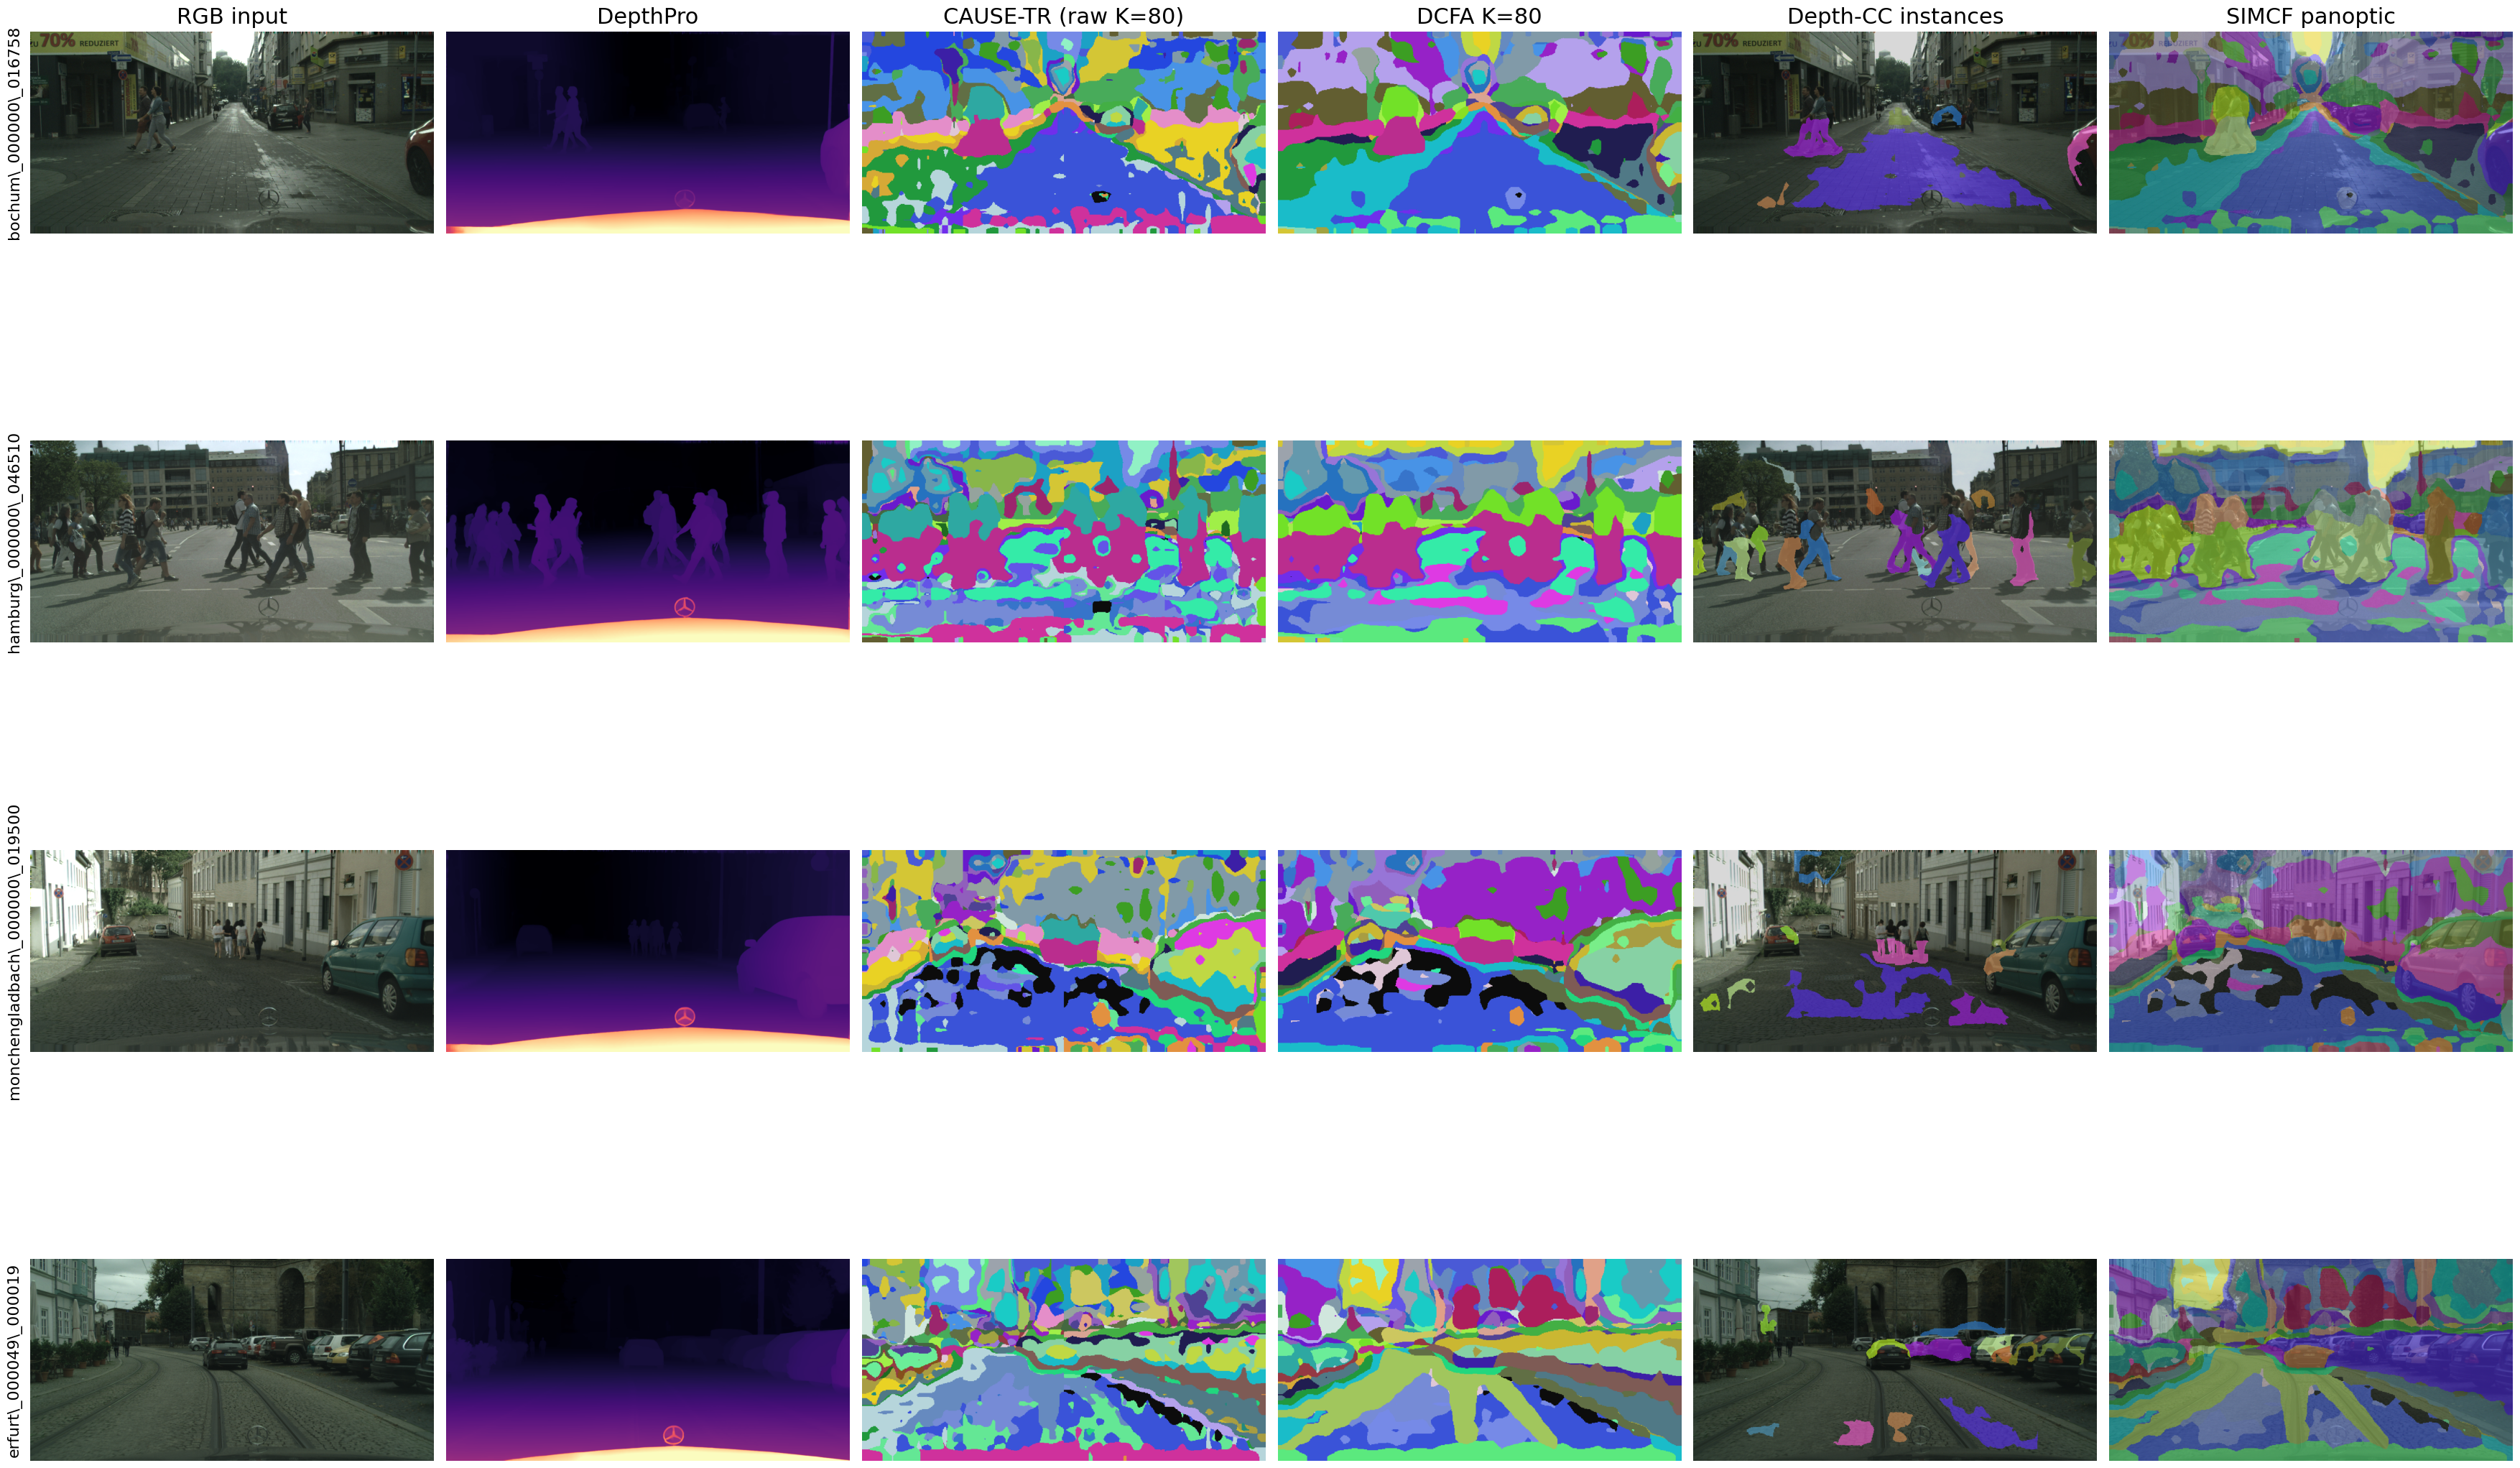
\includegraphics[width=\textwidth]{../figures/paper_ready/fig5_stage1_trace_composite.png}
\caption{Stage-1 pseudo-label trace on four Cityscapes train frames with panels ordered RGB, DepthPro depth, raw $K{=}80$ clusters, DCFA-adjusted $K{=}80$, depth-CC instances overlay, and SIMCF-filtered panoptic overlay.}
\label{fig:supp_real_data_flow}
\end{figure}

\subsection{Cross-Dataset Qualitative Behavior}
\label{sec:supp:cross_dataset_qualitative}

Once Stage-1 supervision is in place, the trained Stage-3 network is evaluated on held-out driving domains under the protocol of Section~\ref{sec:exp:generalization}. Figure~\ref{fig:supp_cross_dataset} extends the quantitative transfer numbers in Table~\ref{tab:transfer} into the image domain, with three frames drawn from Cityscapes, KITTI, Mapillary Vistas v2, and Waymo V2. Stuff and thing colors are produced under the Cityscapes-27 Hungarian alignment that the PQ metric uses, so each row is comparable to every other row.

\begin{figure}[!htbp]
\centering
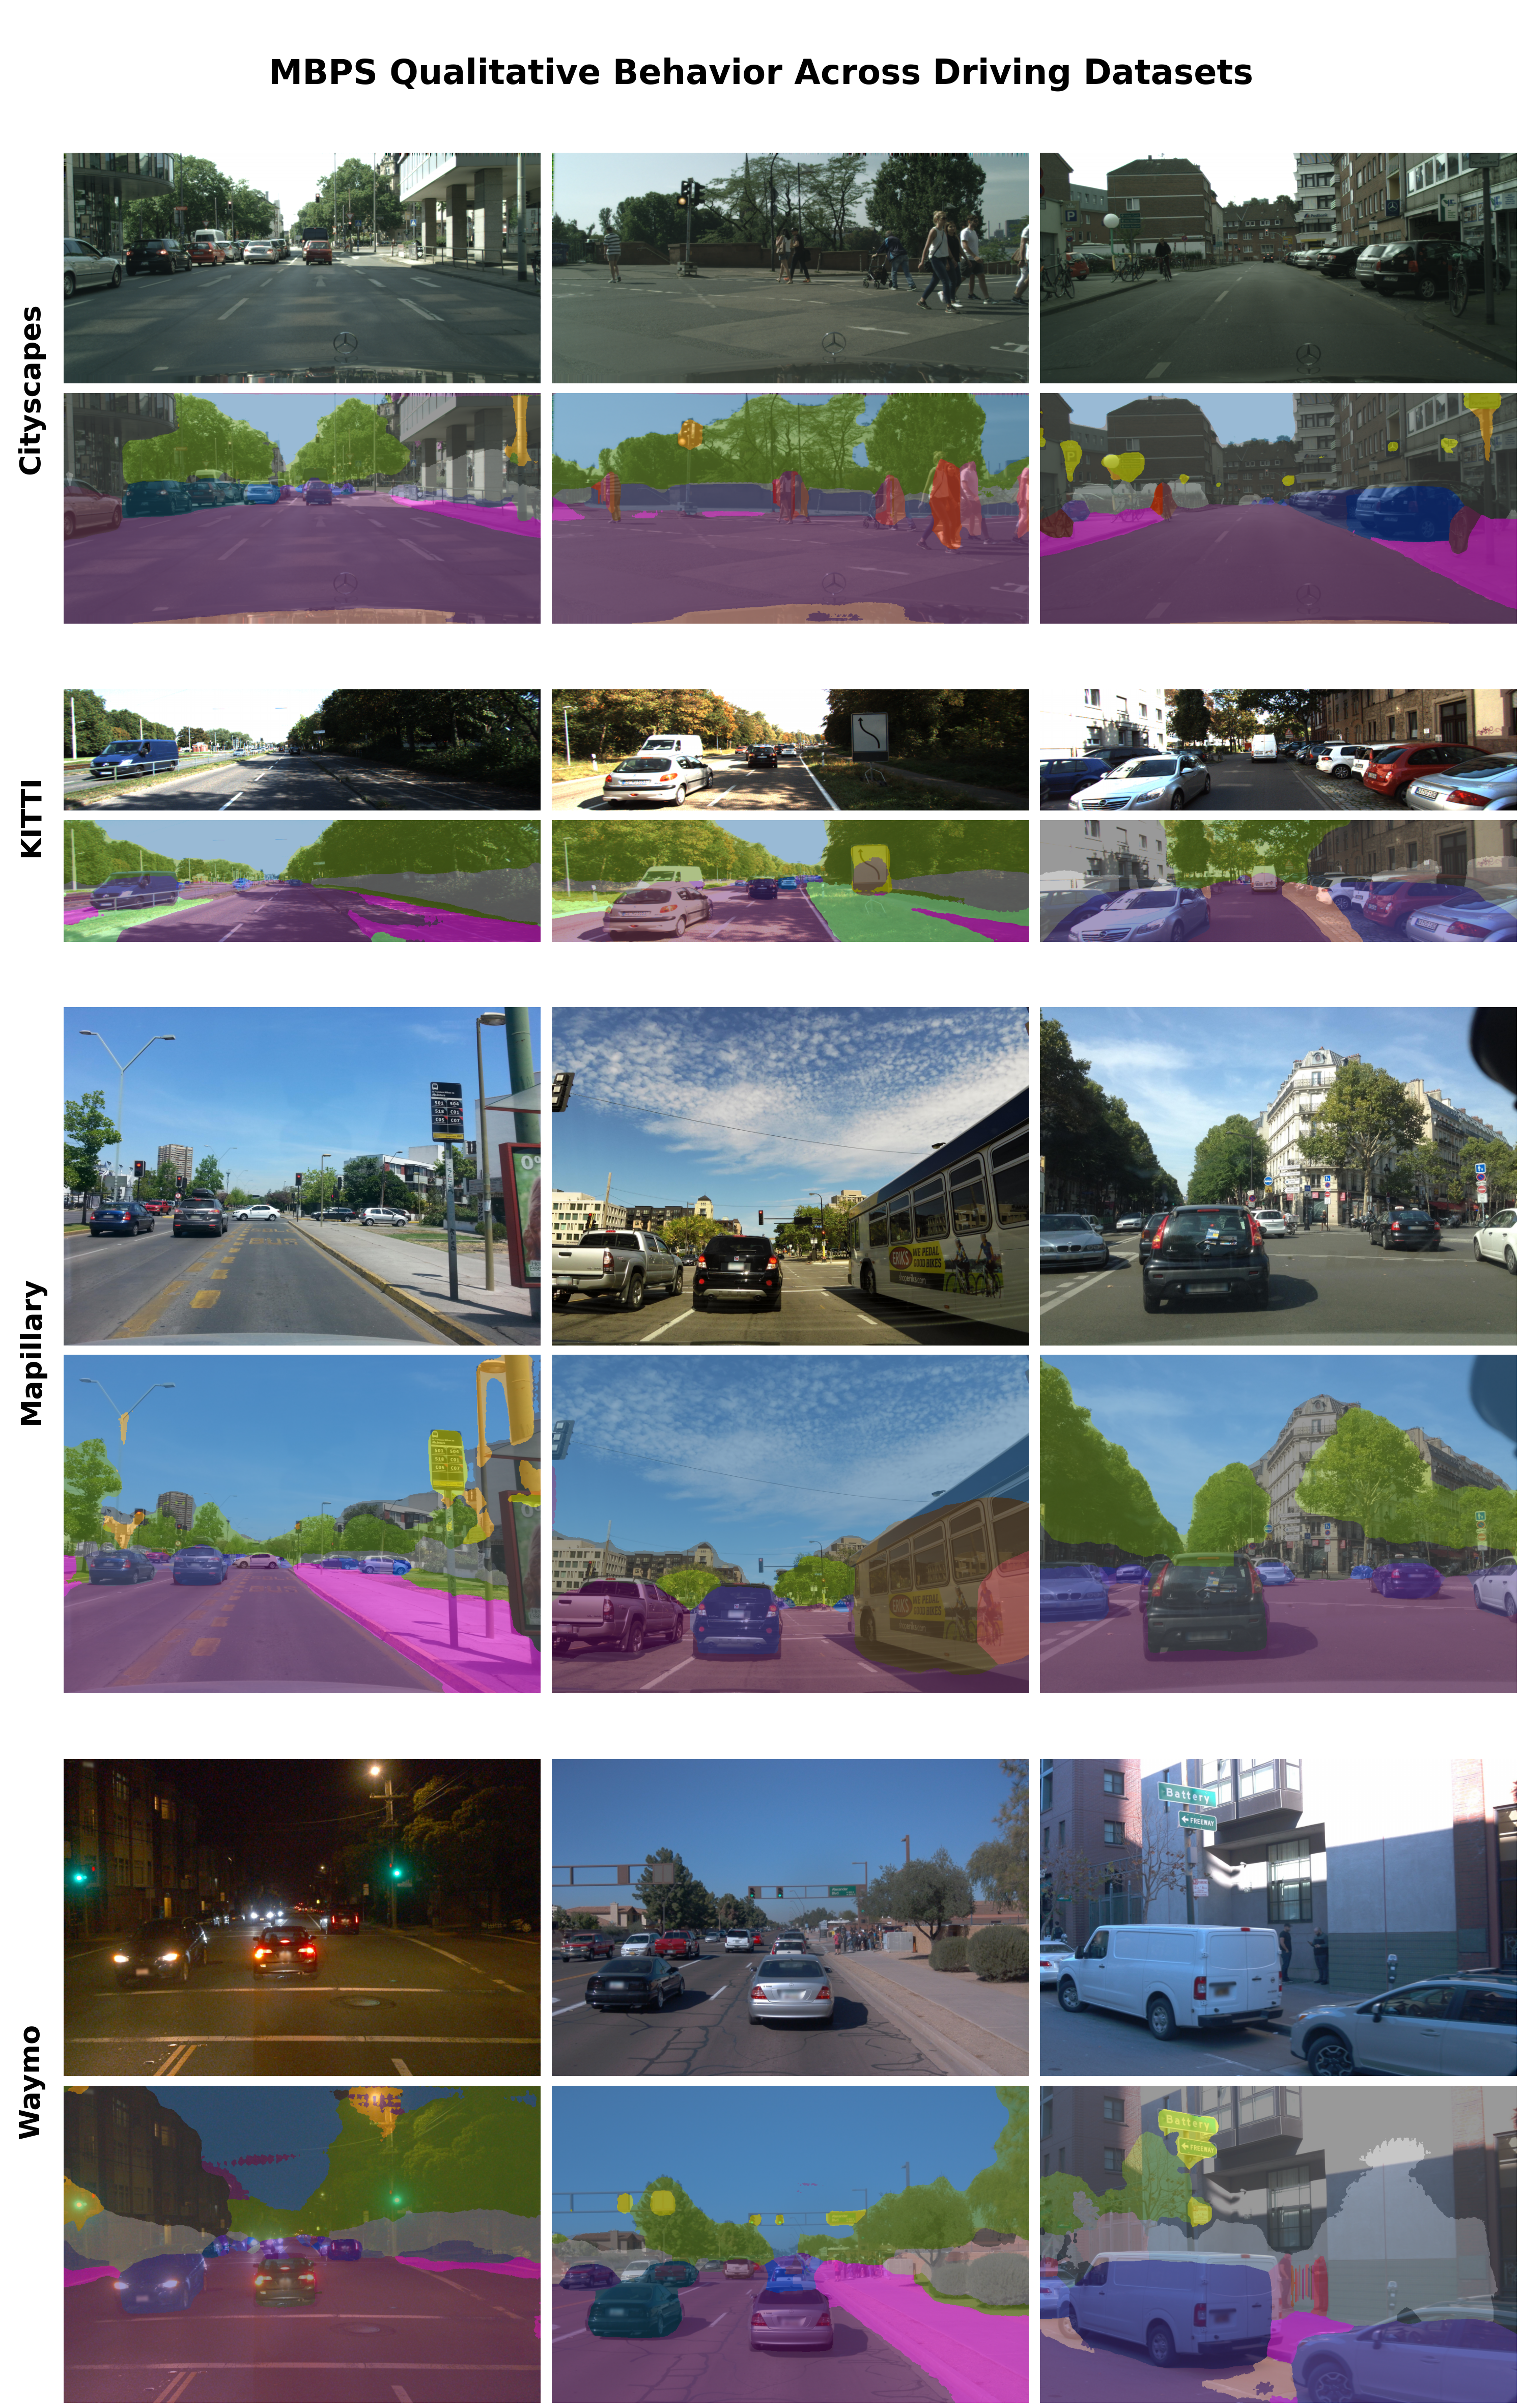
\includegraphics[width=0.92\linewidth]{../figures/paper_ready/supp_qualitative/option_1_cross_dataset_qualitative.png}
\caption{MBPS panoptic predictions on three held-out images from each of Cityscapes, KITTI, Mapillary Vistas v2, and Waymo V2 rendered under the Cityscapes-27 alignment.}
\label{fig:supp_cross_dataset}
\end{figure}

The same alignment supports a like-for-like comparison against the CUPS~\cite{hahn2025cups} baseline. Figure~\ref{fig:supp_ablation_viz} pairs the released CUPS checkpoint with our Stage-3 model on one frame from each of the four domains.

\begin{figure}[!htbp]
\centering
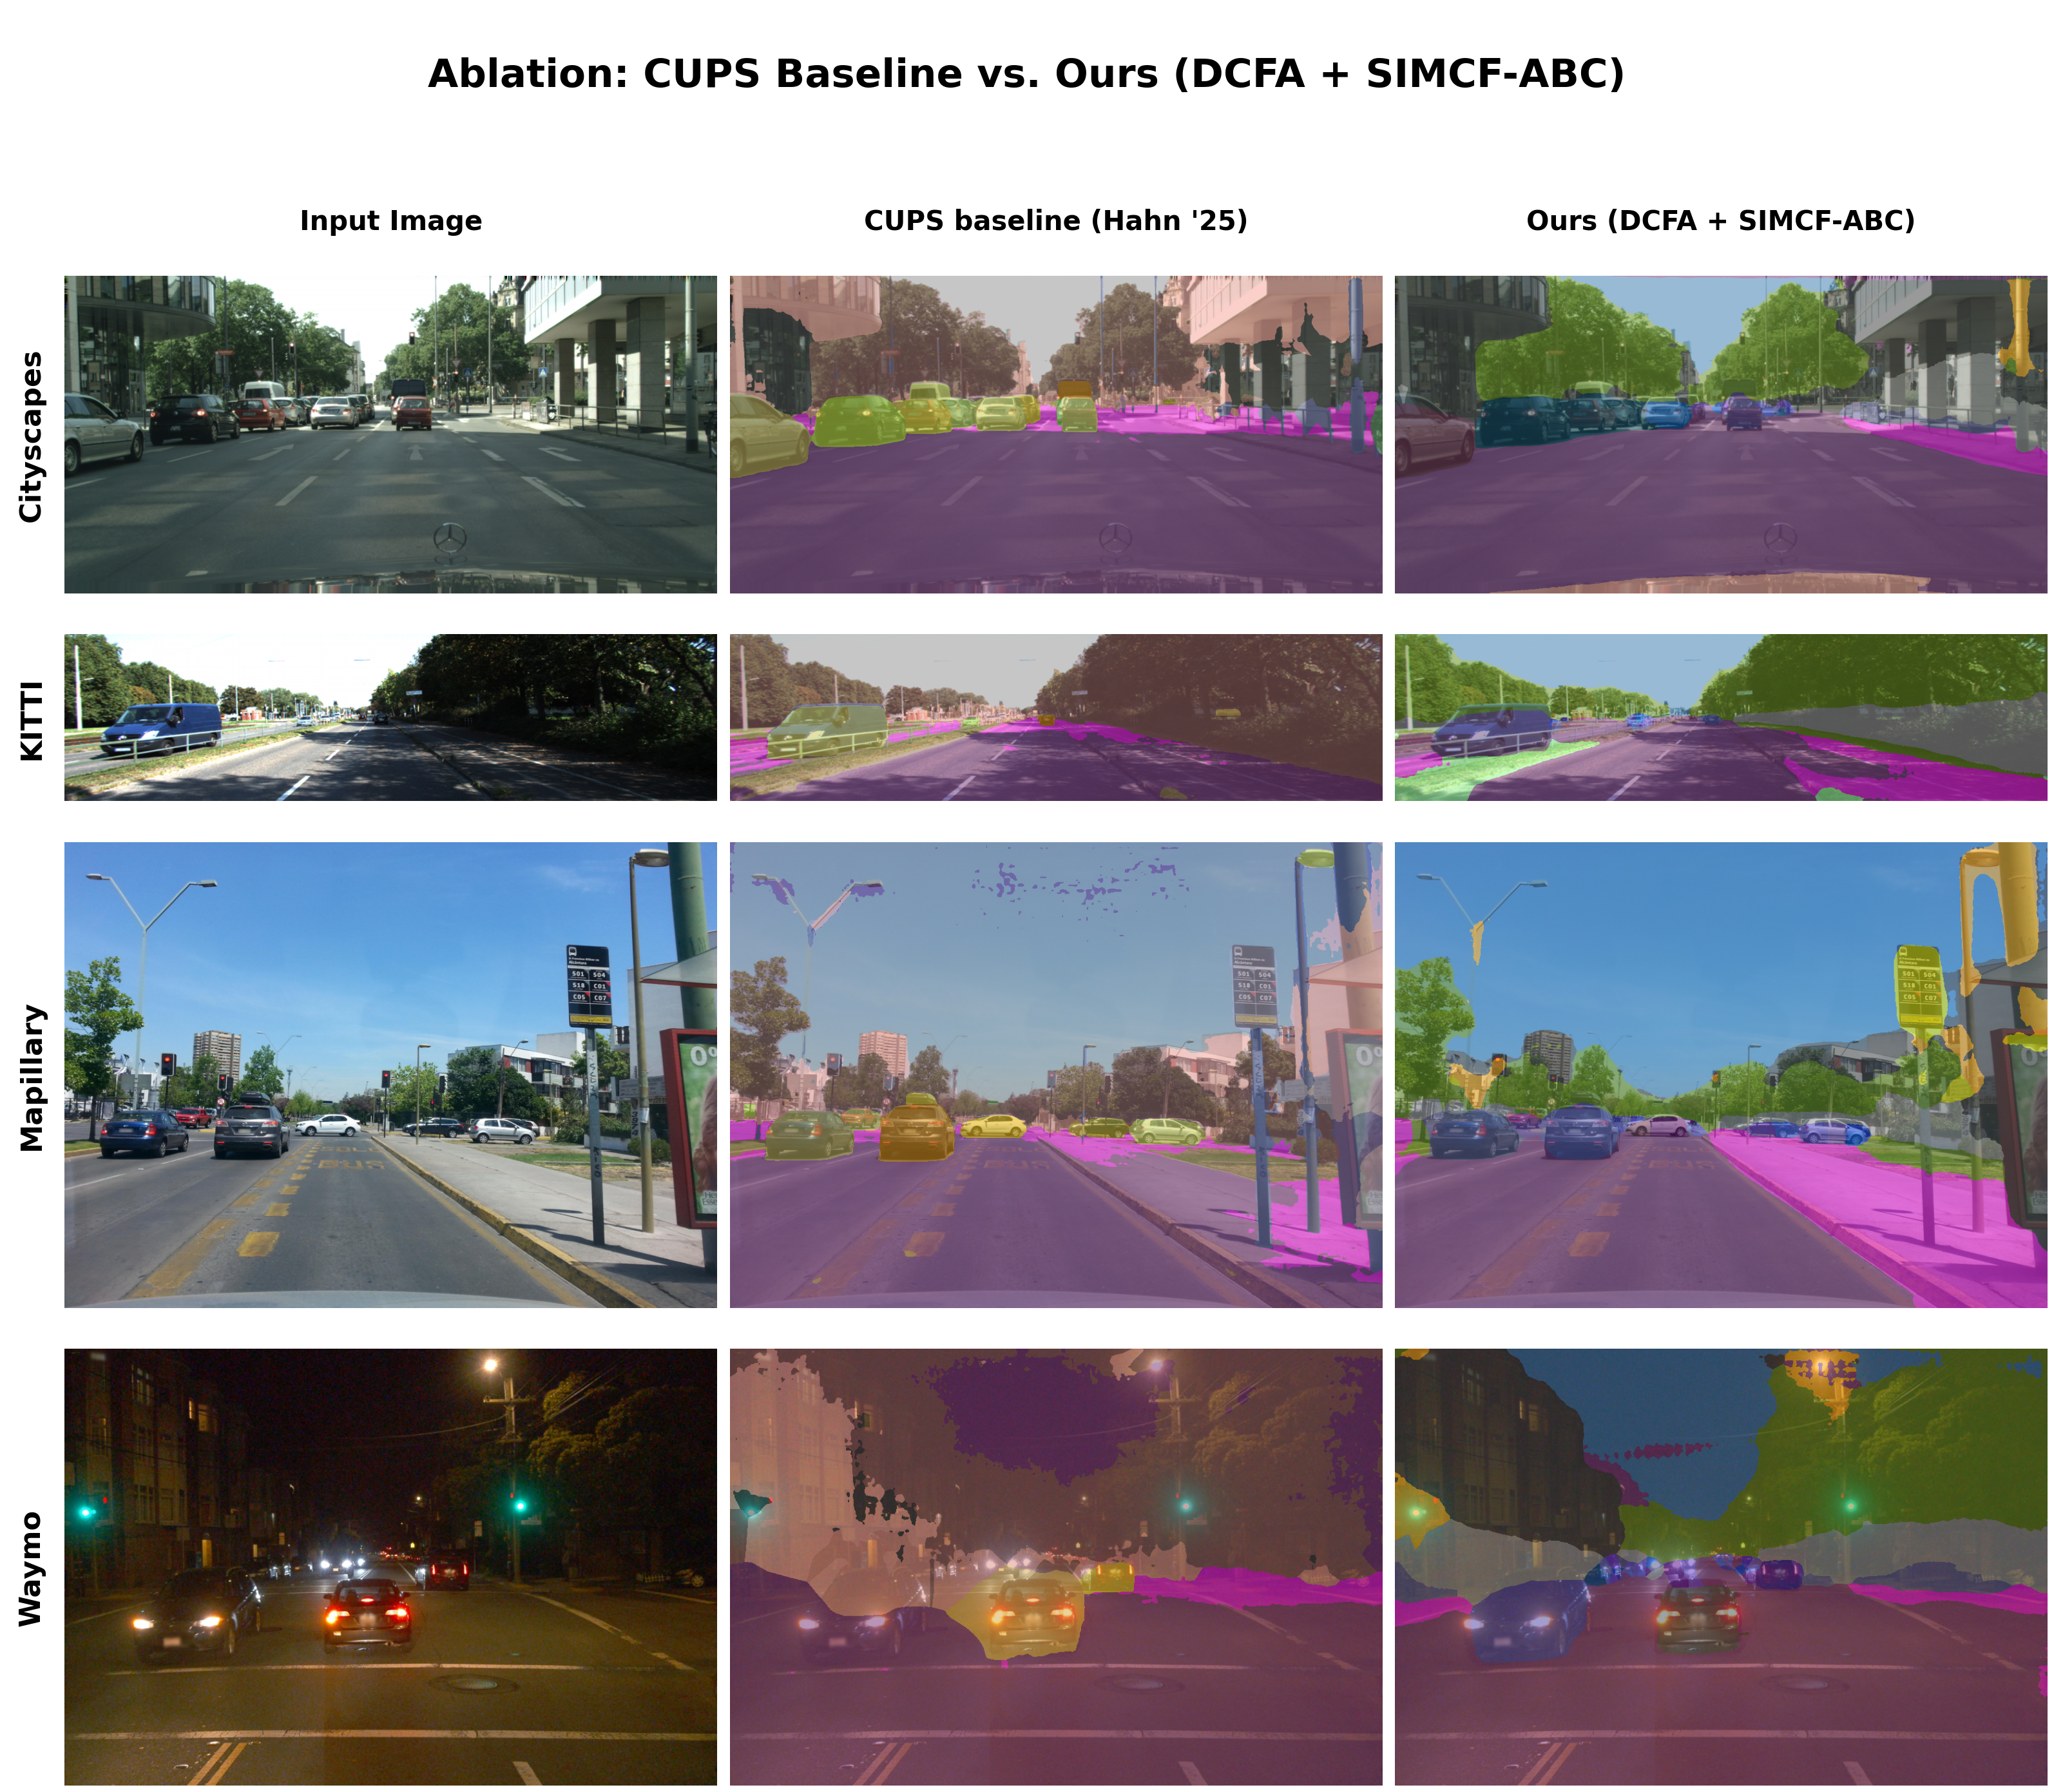
\includegraphics[width=0.92\linewidth]{../figures/paper_ready/supp_qualitative/option_2_ablation_viz.png}
\caption{CUPS and MBPS panoptic predictions on one held-out image from each of Cityscapes, KITTI, Mapillary Vistas v2, and Waymo V2.}
\label{fig:supp_ablation_viz}
\end{figure}

\subsection{Rendering Protocol}
\label{sec:supp:visualization}

The CUPS-vs-MBPS panels above and every other overlay in this appendix share a single rendering convention. Raw pseudo-cluster IDs are projected to the 27-class Cityscapes color palette through the same Hungarian assignment that the PQ metric applies. Each thing instance then receives a color drawn from a shuffled \texttt{tab20} categorical palette, blended at 45\% with its semantic-class color.

%=========================================================================
\section{Implementation Details}
\label{sec:supp:impl}
%=========================================================================

This appendix extends Section~\ref{sec:exp:setup} with the full data, evaluation, hyperparameter, optimizer, augmentation, and hardware configuration used for every reported result.

\subsection{Datasets and Evaluation Protocol}
\label{sec:supp:impl:data}

Pseudo-label generation and panoptic network training use only the 2{,}975 unlabeled Cityscapes train images~\cite{cordts2016cityscapes}. Evaluation is on Cityscapes val (500 images) under the 27-class CAUSE~\cite{kim2024cause} pseudo-vocabulary with a Hungarian map to the 27-class Cityscapes label space (\texttt{NUM\_CLASSES=27} in the official CUPS protocol~\cite{hahn2025cups}). The 27-class evaluation taxonomy includes the 19 standard semantic-segmentation classes together with parking, rail track, guard rail, bridge, tunnel, polegroup, caravan, and trailer. Cross-dataset transfer follows the CUPS~\cite{hahn2025cups} protocol on KITTI~\cite{geiger2012kitti}, Waymo V2~\cite{sun2020waymo}, and Mapillary Vistas v2~\cite{neuhold2017mapillary}.

\subsection{Stage-1: Pseudo-Label Generation}
\label{sec:supp:impl:stage1}

Stage-1 produces semantic and instance pseudo-labels from frozen, self-supervised priors. We freeze the DINOv2 ViT-B/14 backbone~\cite{oquab2024dinov2} and the CAUSE-TR head~\cite{kim2024cause}, which together produce a 90-dimensional concept-clusterbook code per pixel.

DCFA is a two-hidden-layer MLP of width $h{=}384$ acting on the concatenated input $[z_u; e(d_u)] \in \mathbb{R}^{106}$, where $e(d_u)$ is a 16-D sinusoidal embedding of monocular depth, and contributes about 225K trainable parameters. The training objective combines a depth-correlation term and $\lambda_p \mathcal{L}_\text{preserve}$ with $\lambda_p{=}20$, anchoring the residual update to identity at initialisation. We optimize with AdamW (learning rate $10^{-3}$, weight decay $10^{-4}$) for 10K iterations at batch size 32, sampling 1024 pixels and 1024 pixel pairs per image. DCFA training completes in roughly one hour on a single GTX 1080 Ti.

We then fit $k{=}80$ centroids on L2-normalised DCFA-adjusted CAUSE-TR codes over the 2{,}975 Cityscapes train images using \texttt{scikit-learn} mini-batch $k$-means (batch 4096, 100 iterations, fixed random seed). The resulting centroids are saved once and reused throughout the rest of the pipeline.

In parallel, the instance branch consumes frozen monocular depth from DepthPro~\cite{bochkovskii2024depthpro}. We compute depth gradients with $3\times3$ Sobel kernels at threshold $\tau_d{=}0.20$, take 8-neighbour connected components inside thing-eligible semantic regions, drop components below $A_\text{min}{=}1000$ pixels, and apply three iterations of $3\times3$ dilation.

SIMCF then reconciles the two branches. It uses a feature similarity threshold $\tau_\text{sim}{=}0.85$ and a depth-implausibility multiplier $\eta{=}2.5$, applying adjacent-proposal merging (Step~B) before depth-implausibility void rejection (Step~C).

\subsection{Stage-2: Panoptic Bootstrapping}
\label{sec:supp:impl:stage2}

Cascade Mask R-CNN~\cite{cai2018cascade} with three cascade stages on a frozen DINOv3 ViT-B/16 backbone~\cite{simeoni2025dinov3} (no backbone fine-tuning). 8K optimizer steps, batch size 8 (4 per GPU), AdamW (lr $10^{-4}$, weight decay $0.05$, $\beta_1{=}0.9$, $\beta_2{=}0.999$), cosine schedule with 500-step linear warmup. Loss includes DropLoss~\cite{wang2023cutler} ($\lambda_\text{drop}{=}1.0$) and self-enhanced copy-paste augmentation. Augmentation: random horizontal flip, random scale jitter $[0.5, 2.0]$, random crop $1024\times1024$, copy-paste with probability 0.5, photometric jitter (brightness $\pm$0.2, contrast $\pm$0.2, saturation $\pm$0.2). Wall-clock: $\approx 12$ hours on $2\times$ NVIDIA GTX 1080 Ti with PyTorch DistributedDataParallel.

\subsection{Stage-3: EMA Self-Training}
\label{sec:supp:impl:stage3}

After Stage-2 converges, we run three EMA self-training rounds of 5K optimizer steps each with EMA coefficient 0.999. A three-scale teacher (scales $\{0.75, 1.0, 1.25\}$) supplies class-aware confidence thresholds (foreground 0.4, background 0.3). We reuse the Stage-2 augmentation pipeline and optimizer family with a base learning rate of $5\times10^{-5}$ at the start of each round under a per-round cosine schedule. Stage-3 takes roughly 16 wall-clock hours on $2\times$ GTX 1080 Ti.

\subsection{Hardware and Wall-Clock Budget}
\label{sec:supp:impl:hardware}

Aggregating the per-stage budgets above, all training runs on $2\times$ NVIDIA GTX 1080 Ti GPUs (consumer-grade, 11 GB VRAM each) under PyTorch DistributedDataParallel. Stage-1 generation accounts for roughly 2 GPU-hours, Stage-2 bootstrapping for 24 GPU-hours (12 wall-clock on 2 GPUs), and Stage-3 self-training for 32 GPU-hours (16 wall-clock), giving an aggregate of 58 GPU-hours. The pipeline therefore runs end-to-end on consumer-grade hardware, without the calibrated stereo rigs or synchronized video that CUPS~\cite{hahn2025cups} requires at pseudo-label time.

\subsection{DCFA Loss Definitions}
\label{sec:supp:impl:dcfa_loss}

Let $\mathcal{U}$ denote the set of $|\mathcal{U}| = 1024$ pixels sampled per image and $\mathcal{P}$ the set of $|\mathcal{P}| = 1024$ pixel pairs sampled from $\mathcal{U}$. Then
\begin{align*}
\mathcal{L}_\text{corr} &= \tfrac{1}{|\mathcal{P}|}\!\!\sum_{(i,j)\in\mathcal{P}} \mathcal{K}_{\sigma_d}(D_i, D_j)\,\big(1 - \cos(\tilde z_i, \tilde z_j)\big), \\
\mathcal{L}_\text{preserve} &= \tfrac{1}{|\mathcal{U}|} \sum_{u \in \mathcal{U}} \|\tilde z_u - z_u\|_2^2,
\end{align*}
where $\mathcal{K}_{\sigma_d}$ is the DepthG~\cite{sick2024depthg} depth-similarity kernel with bandwidth $\sigma_d=0.5$. Both losses are averaged over the sampled set per image, then averaged over the minibatch.

\subsection{Reproducibility Notes}
\label{sec:supp:impl:repro}

All random seeds are fixed at the beginning of each stage (DCFA training seed $42$, $k$-means seed $0$, Stage-2/3 dataloader seed $42$). We implement the pipeline in Python 3.10 with PyTorch 2.1, Detectron2 0.6, and CUDA 11.8. Stage-1 pseudo-labels and Stage-2/3 checkpoints accompany the code release.

%=========================================================================
\section{SIMCF Step Ablation and Threshold Sensitivity}
\label{sec:supp:simcf_sweep}
%=========================================================================

SIMCF takes the raw candidate pair $(S_x^0, I_x^0)$ from the Stage-1 generator and produces filtered pseudo-labels $(\hat S_x, \hat I_x)$ through three composable steps that share two thresholds, $\tau_\text{sim}$ for adjacent-proposal feature merging in Step~B and $\eta$ for depth-implausibility void rejection in Step~C. The three steps are A (intra-instance majority vote), B (cosine-merge), and C (depth void). Both Algorithm~\ref{alg:simcf} and the per-step ablation that follows reference a fixed over-cluster-to-concept map $\phi : \{1, \dots, 80\} \to \{1, \dots, 27\}$, which we define here before stating the algorithm.

\paragraph{The over-cluster-to-concept map $\phi$.}
\label{sec:supp:impl:phi}
The source side of $\phi$ is the set of 80 $k$-means cluster centroids fitted on the DCFA-adjusted 90-D semantic codes of Cityscapes train (Section~\ref{sec:method:baseline}). The target side is the 27 concept prototypes inside the frozen CAUSE-TR head~\cite{kim2024cause}. CAUSE-TR was trained without human annotation, on Cityscapes train images using only the self-supervised concept-coherence objective, so its 27 prototypes form an internally-discovered partition of the latent space rather than a label space. For each $k \in \{1, \dots, 80\}$, $\phi(k) = \arg\min_{c \in \{1, \dots, 27\}} \|\mu_k - p_c\|_2$, where $\mu_k$ is the $k$-th $k$-means centroid and $p_c$ is the $c$-th CAUSE concept prototype, both in the 90-D code space. The thing-stuff partition over the 27 CAUSE concepts (8 thing categories, 19 stuff categories) is fixed by CAUSE-TR's pretraining and read off the frozen head. The only ground-truth-derived component anywhere in the pipeline is the Hungarian map between the 27 CAUSE concept prototypes and the 27 Cityscapes evaluation classes, computed once at metric time (Section~\ref{sec:exp:setup}); it never feeds back into Stage-1 generation, the panoptic network, or any operating hyperparameter.

With $\phi$ in place, Algorithm~\ref{alg:simcf} states the full SIMCF procedure, after which we isolate the per-step contribution of A, B, and C and characterise the sensitivity of the two thresholds.

\begin{algobox}[H]
\caption{SIMCF$(S_x^0,I_x^0,D,\phi,v;\tau_\text{sim},\eta)$. $\phi$ maps over-clusters to the 27-class CAUSE taxonomy, and $v$ is dense DINOv3 features.}
\label{alg:simcf}
\begin{enumerate}
\setlength{\itemsep}{0pt}
\item $(\hat S_x,\hat I_x) \gets (S_x^0,I_x^0)$
\item \textit{for each} instance region $R_k=\{p:\hat I_x(p)=k\}$ \textit{do}
\item \quad $c_k \gets \arg\max_c |\{p\in R_k:\phi(\hat S_x(p))=c\}|$
\item \quad $s_k \gets \arg\max_s |\{p\in R_k:\hat S_x(p)=s,\ \phi(s)=c_k\}|$
\item \quad \textit{for each} $p\in R_k$ with $\phi(\hat S_x(p))\ne c_k$ \textit{do} $\hat S_x(p)\gets s_k$
\item \textit{for each} adjacent proposal pair $(a,b)$ in $\hat I_x$ \textit{do}
\item \quad compute mean features $\bar v_a,\bar v_b$ over $R_a,R_b$
\item \quad \textit{if} $c_a=c_b$ and $\cos(\bar v_a,\bar v_b)>\tau_\text{sim}$ \textit{then} merge $R_a$ and $R_b$ in $\hat I_x$
\item \textit{for each} pseudo-class $c$ \textit{do}
\item \quad $P_c\gets\{p:\phi(\hat S_x(p))=c\}$;\quad $(\mu_c,\sigma_c)\gets(\operatorname{mean}D(P_c),\operatorname{std}D(P_c))$
\item \textit{for each} pixel $p$ \textit{do}
\item \quad $c\gets\phi(\hat S_x(p))$
\item \quad \textit{if} $|D(p)-\mu_c|>\eta\sigma_c$ \textit{then} $\hat S_x(p)\gets\mathrm{void}$; $\hat I_x(p)\gets0$
\item \textit{return} $(\hat S_x,\hat I_x)$
\end{enumerate}
\end{algobox}

Table~\ref{tab:simcf_step_ablation} reports pseudo-label PQ on Cityscapes train ($N{=}2975$) with steps incrementally enabled. All variants share the DCFA-conditioned $K{=}80$ semantic source and DepthPro $\tau_d{=}0.20$ instance proposals.

\begin{table}[!htbp]
\caption{Step-by-step SIMCF contribution to pseudo-label PQ on Cityscapes train under the 19-class many-to-one cluster-to-class mapping.}
\label{tab:simcf_step_ablation}
\centering
\small
\setlength{\tabcolsep}{6pt}
\begin{tabular}{l c c c c c c}
\toprule
Setting & PQ & $\Delta$PQ & PQ$^\text{st}$ & PQ$^\text{th}$ & mIoU & Ignore (\%) \\
\midrule
DCFA only (no SIMCF)        & 25.22 & ---     & 33.99 & 13.16 & 56.16 & 0.00 \\
\, $+$ SIMCF-A              & 25.22 & $+$0.00 & 33.99 & 13.16 & 56.16 & 0.00 \\
\, $+$ SIMCF-A$+$B          & 25.84 & $+$0.62 & 33.99 & 14.64 & 56.16 & 0.00 \\
\, $+$ SIMCF-A$+$B$+$C      & \textbf{25.85} & \textbf{$+$0.63} & 33.96 & \textbf{14.70} & 56.22 & 0.84 \\
\bottomrule
\end{tabular}
\end{table}

Step~B carries the entire PQ$^\text{th}$ gain. The instance map is touched only by Step~B, where per-image instance count drops from 16.2 to 7.0 and median instance size rises from 6{,}372 to 16{,}413 pixels. These statistics confirm the depth over-fragmentation behaviour described in Section~\ref{sec:method}. Step~A is inert on DCFA-conditioned codes because within-instance cluster purity is already high, and Step~C trades 0.84\% void for marginal stuff cleanup. Because pseudo-label PQ lower-bounds Stage-3 trained PQ, the $+0.63$ pseudo-label gain is consistent with the $+3.07$ trained-PQ contribution reported in Table~\ref{tab:main}.

Having localised the gain to Step~B, we next ask whether the specific values $\tau_\text{sim}{=}0.85$ and $\eta{=}2.5$ are themselves load-bearing. We sweep both thresholds within roughly $\pm 12\%$ of the paper setting and re-evaluate Stage-1 pseudo-label quality on the full Cityscapes train set under the CUPS~\cite{hahn2025cups} 27-class protocol. The sweep is therefore directly comparable to the Stage-1 numbers in Table~\ref{tab:components} and not to the trained-PQ numbers elsewhere in the main paper.

\begin{table}[!htbp]
\caption{Stage-1 pseudo-label quality on Cityscapes train as $\tau_\text{sim}$ and $\eta$ are swept around the paper setting.}
\label{tab:simcf_sensitivity}
\centering
\small
\setlength{\tabcolsep}{6pt}
\begin{tabular}{l c c c c c c}
\toprule
Setting & $\tau_\text{sim}$ & $\eta$ & PQ & SQ & RQ & mIoU \\
\midrule
tighter           & 0.75 & 2.0 & 25.98 & 58.79 & 34.55 & 56.08 \\
baseline (paper)  & 0.85 & 2.5 & 25.87 & 58.38 & 34.83 & 56.17 \\
looser            & 0.95 & 3.0 & 25.27 & 57.63 & 34.10 & 56.22 \\
\bottomrule
\end{tabular}
\end{table}

Pseudo-label PQ varies within a 0.71-point band (25.27 to 25.98) across the sweep, well inside the $+1.31$ PQ gap from the raw $K{=}80$ baseline (24.54) to Both (25.85) reported in main-paper Table~\ref{tab:components}. Tighter thresholds slightly improve PQ and looser thresholds degrade modestly, so the mechanism is robust to moderate threshold perturbation.

%=========================================================================
\section{Depth Model Ablation}
\label{sec:supp:depth}
%=========================================================================

Holding the SIMCF threshold at the value selected in Section~\ref{sec:supp:simcf_sweep}, we vary the monocular depth estimator and the gradient threshold $\tau$. Three estimators are compared, namely SPIdepth, Depth-Anything v3~\cite{lin2025da3}, and DepthPro~\cite{bochkovskii2024depthpro}. Rows mix the raw $K{=}80$ semantic map and the DCFA semantic map, so reading them jointly isolates mask quality from recognition quality and fixes the training-data configuration used in Section~\ref{sec:exp:main}. The diagnostics are computed on Cityscapes train pseudo-labels at the Stage-1 level, which is distinct from the Cityscapes val numbers reported in Tables~\ref{tab:main}, \ref{tab:components}, and \ref{tab:conditioning} of the main paper.

\begin{table}[!htbp]
\caption{Depth-estimator and gradient-threshold diagnostics on Cityscapes train pseudo-labels.}
\label{tab:depth}
\centering
\small
\setlength{\tabcolsep}{6pt}
\begin{tabular}{l l c c c c}
\toprule
Depth & Sem. & $\tau$ & PQ & SQ & RQ \\
\midrule
SPIdepth & raw $K$=80 & 0.20 & 26.74 & 71.88 & 31.41 \\
DA v3~\cite{lin2025da3} & raw $K$=80 & 0.03 & 27.37 & 73.44 & 35.66 \\
DA v3~\cite{lin2025da3} & DCFA & 0.20 & 26.44 & 61.37 & 35.83 \\
DepthPro~\cite{bochkovskii2024depthpro} & DCFA & 0.01 & 27.81 & 63.07 & 37.40 \\
DepthPro~\cite{bochkovskii2024depthpro} & DCFA & 0.20 & 26.13 & 60.63 & 35.80 \\
\bottomrule
\end{tabular}
\end{table}

PQ alone is not a sufficient diagnostic for the depth branch. The sharper $\tau{=}0.01$ DepthPro setting reaches the strongest standalone PQ, SQ, and RQ, yet yields roughly 57 instances per image with more than half under 1000 pixels. The $\tau{=}0.20$ setting reports lower standalone PQ but produces larger training targets, roughly 22 instances per image, and is the configuration used for panoptic bootstrapping in the main paper. Under the same threshold, DA v3 reaches a similar RQ, so the choice is governed by the training signal produced by the depth branch rather than by the stuff-thing aggregate split.

%=========================================================================
\section{Out-of-Distribution Sanity Checks}
\label{sec:supp:ood}
%=========================================================================

Beyond the in-domain cross-dataset transfer reported in the main paper on KITTI~\cite{geiger2012kitti}, Waymo V2~\cite{sun2020waymo}, and Mapillary v2~\cite{neuhold2017mapillary} (Section~\ref{sec:exp:generalization}), two further sanity checks probe vocabularies outside that range. MOTS~\cite{voigtlaender2019mots} isolates a thing-only label space whose vocabulary is a subset of Cityscapes-things, and COCO-Stuff-27~\cite{caesar2018coco} supplies a vocabulary-mismatched object-centric setting whose 27 classes overlap only partially with Cityscapes-27. Table~\ref{tab:cocooo} reports both.

\begin{table}[!htbp]
\caption{Out-of-distribution checks on MOTS and COCO-Stuff-27. Values are percentages.}
\label{tab:cocooo}
\centering
\footnotesize
\setlength{\tabcolsep}{6pt}
\begin{tabular}{l c c c c}
\toprule
Dataset (OOD) & \# img & PQ & SQ & RQ \\
\midrule
MOTS~\cite{voigtlaender2019mots} thing-only & 2{,}862 & 61.10 & 88.71 & 65.80 \\
\quad CUPS~\cite{hahn2025cups} ref. & --- & 86.4 & 86.4 & 76.9 \\
COCO-Stuff-27~\cite{caesar2018coco} vocab.\ mismatch & 1{,}000 & \phantom{0}7.83 & 38.55 & 10.06 \\
\bottomrule
\end{tabular}
\end{table}

On MOTS the Stage-3 network reaches 61.10 PQ with SQ 88.71, showing that mask geometry transfers to a thing-only vocabulary on KITTI-style sequences when the label space drops from 27 classes to a thing-only subset. The gap to the CUPS~\cite{hahn2025cups} reference is recognition-driven, with RQ 65.80 against 76.9, and vocabulary granularity accounts for the difference. On COCO-Stuff-27 the aggregate falls to 7.83 PQ, dominated by categories absent from a Cityscapes-derived pseudo-label space, including kitchenware, sports gear, and food. The result delineates the vocabulary boundary of in-domain training, where coverage of object-centric vocabularies outside the Cityscapes pseudo-space is set by the generator's vocabulary itself.

%=========================================================================
\section{Per-Class Cityscapes Metrics}
\label{sec:supp:perclass}
%=========================================================================

Within the in-domain Cityscapes vocabulary, the per-class PQ, SQ, and RQ profile of the final trained network is given in Table~\ref{tab:perclass}. Reporting follows the CUPS~\cite{hahn2025cups} 27-class evaluation protocol with Hungarian matching from the $K{=}80$ pseudo-vocabulary to the 27-class Cityscapes label space.

\begin{table}[!htbp]
\caption{Per-class Cityscapes validation PQ, SQ, and RQ for the final trained network. Values are percentages.}
\label{tab:perclass}
\centering
\small
\setlength{\tabcolsep}{6pt}
\resizebox{\textwidth}{!}{%
\begin{tabular}{l c c c l c c c l c c c}
\toprule
Class & PQ & SQ & RQ & Class & PQ & SQ & RQ & Class & PQ & SQ & RQ \\
\midrule
road & 93.0 & 95.0 & 97.9 & tunnel & 0.0 & 0.0 & 0.0 & rider & 22.9 & 62.6 & 36.6 \\
sidewalk & 62.4 & 78.5 & 79.5 & pole & 2.0 & 72.3 & 2.8 & car & 70.7 & 88.7 & 79.7 \\
parking & 0.0 & 0.0 & 0.0 & polegroup & 0.0 & 0.0 & 0.0 & truck & 62.6 & 83.8 & 74.7 \\
rail track & 8.4 & 67.2 & 12.5 & traffic light & 6.2 & 60.3 & 10.3 & bus & 76.7 & 90.8 & 84.4 \\
building & 83.5 & 85.7 & 97.5 & traffic sign & 37.2 & 65.9 & 56.4 & caravan & 0.0 & 0.0 & 0.0 \\
wall & 32.3 & 67.7 & 47.8 & vegetation & 84.7 & 85.7 & 98.8 & trailer & 0.0 & 0.0 & 0.0 \\
fence & 20.3 & 63.0 & 32.1 & terrain & 35.7 & 73.4 & 48.6 & train & 77.2 & 88.7 & 87.0 \\
guard rail & 0.0 & 0.0 & 0.0 & sky & 86.1 & 89.9 & 95.7 & motorcycle & 0.1 & 100.0 & 0.1 \\
bridge & 17.2 & 64.5 & 26.7 & person & 13.4 & 71.4 & 18.7 & bicycle & 39.0 & 77.2 & 50.5 \\
\bottomrule
\end{tabular}
}
\end{table}

The 35.83 PQ aggregate is carried by twenty active classes. Large stuff regions and large vehicles all exceed 70 PQ, with road, sky, vegetation, and building above 80, since frozen semantic codes produce coherent regions and depth boundaries align with object extent. Six classes (parking, guard rail, tunnel, polegroup, caravan, and trailer) lie outside the standard Cityscapes-19 panoptic benchmark and receive few positive examples in the $K{=}80$ over-cluster vocabulary, while motorcycle matches a single near-perfect instance with SQ 100. Restricting the average to the standard Cityscapes-19 panoptic classes is therefore the protocol-comparable reading of the headline.

The same table exposes the recognition bottleneck for closely-spaced object classes. Person reaches SQ 71.4 and rider SQ 62.6, both above the 60-point band that classifies the per-class match as geometrically correct, while their RQ values, 18.7 and 36.6, are recognition-limited by depth-based instance separation on co-planar pedestrian crowds. Section~\ref{sec:conclusion} returns to the co-planar pedestrian regime as the principal recognition-side residual.

These per-class recognition limits motivate the feature-guided merge step (Step~B) of SIMCF, whose two aggregate measurements close the per-class picture. The average pseudo-instance count per image drops from 44 before the merge to 22 after. Median instance size grows from 5{,}502 to 14{,}965 pixels, and stuff contamination falls from 50.7\% to 28.0\%. Many depth gradients are intra-object surface changes, and merging fragments whose semantic identity and dense appearance agree recovers the single-object structure that monocular depth had over-fragmented.

%=========================================================================
\section{Broader Impact}
\label{sec:impact}
%=========================================================================

\noindent Beyond per-class behaviour, the monocular-only design itself reshapes the deployment surface for unsupervised panoptic segmentation. Removing stereo and motion requirements at pseudo-label time broadens the range of imagery to which scene-centric unsupervised panoptic segmentation can be applied, with autonomous-driving and robotic-perception pipelines that ingest monocular footage from phones, dashcams, or fixed cameras as the intended beneficiaries.

The same property changes the deployment surface. Monocular footage is cheaper to acquire and easier to repurpose for surveillance and behavioural-monitoring settings that stereo-based methods could not reach. Released artifacts are restricted to street-scene category training, and person re-identification is outside the evaluated label space.

Two design-level biases warrant explicit calibration. First, the frozen pseudo-label vocabulary inherits any class-imbalance and dataset-bias signal already present in CAUSE-TR's~\cite{kim2024cause} Cityscapes-derived clusterbook, so the six low-population pseudo-classes from Section~\ref{sec:supp:perclass} reflect the source vocabulary that calibration on demographically distinct scenes must account for. Second, depth-based instance separation degrades on co-planar pedestrian crowds, which are over-represented in dense urban settings and may correlate with population density or geography. Calibration of the person-class instance behaviour is therefore a prerequisite for deployment in settings where mispredictions carry operational cost.

Two technical-bias concerns also follow from the design. First, the frozen pseudo-label vocabulary inherits any class-imbalance and dataset-bias signal already present in CAUSE-TR's~\cite{kim2024cause} Cityscapes-derived clusterbook; six dead classes, discussed in the main paper's limitations section, are a direct symptom and would compound on demographically less-represented scenes. Second, depth-based instance separation degrades on co-planar pedestrian crowds, which are over-represented in dense urban settings and may correlate with population density or geography. These limitations should be accounted for before downstream deployment, particularly in settings where the consequences of mispredicted person-class instances are non-trivial.

\end{document}
